% Methodology

\begin{figure}
    \centering
    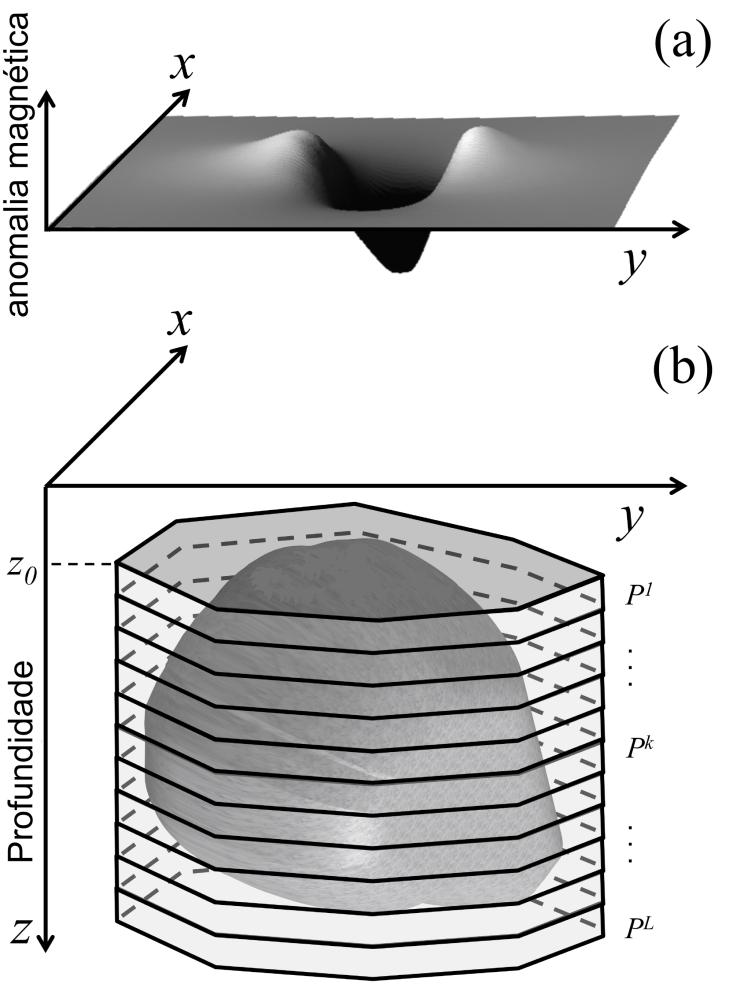
\includegraphics[scale=1]{figures/observed_data.png}
    \caption{Schematic representation (modified from \cite{oliveirajr-barbosa2013}) of (a) total-field anomaly (gray surface) produced by (b) a 3-D anomalous source (dark gray volume). The interpretation model in (b) consists of a set of $L$ vertical, juxtaposed 3-D prisms (light gray) in the vertical direction of a right-handed coordinate system. At the initial iteration, the interpretation model is defined as a vertical cylinder.}
    \label{fig:obs}
\end{figure}

\begin{figure}
    \centering
    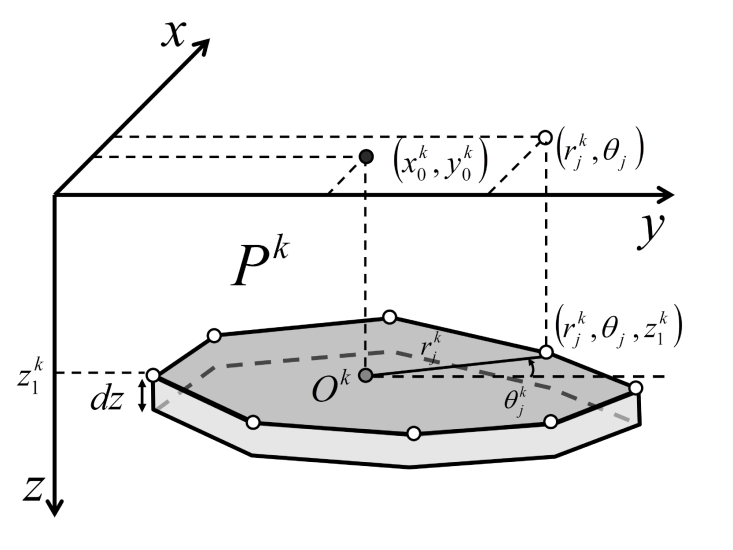
\includegraphics[scale=0.3]{figures/prism_parameters_mod.png}
    \caption{Polygonal cross-section of the $k$th vertical prism described by $V$ vertices (white dots) with radii $r^k_j$, $j = 1, \dots, V$, $k = 1, \dots, L$ , referred to an arbitrary origin $O^k$ (grey dot) with horizontal Cartesian coordinates ($x_0^k$ , $y_0^k$), $k = 1, \dots, L$ , (black dot).}
    \label{fig:prism_parameters}
\end{figure}

% Application to synthetic data - simple model

\begin{figure}
    \centering
    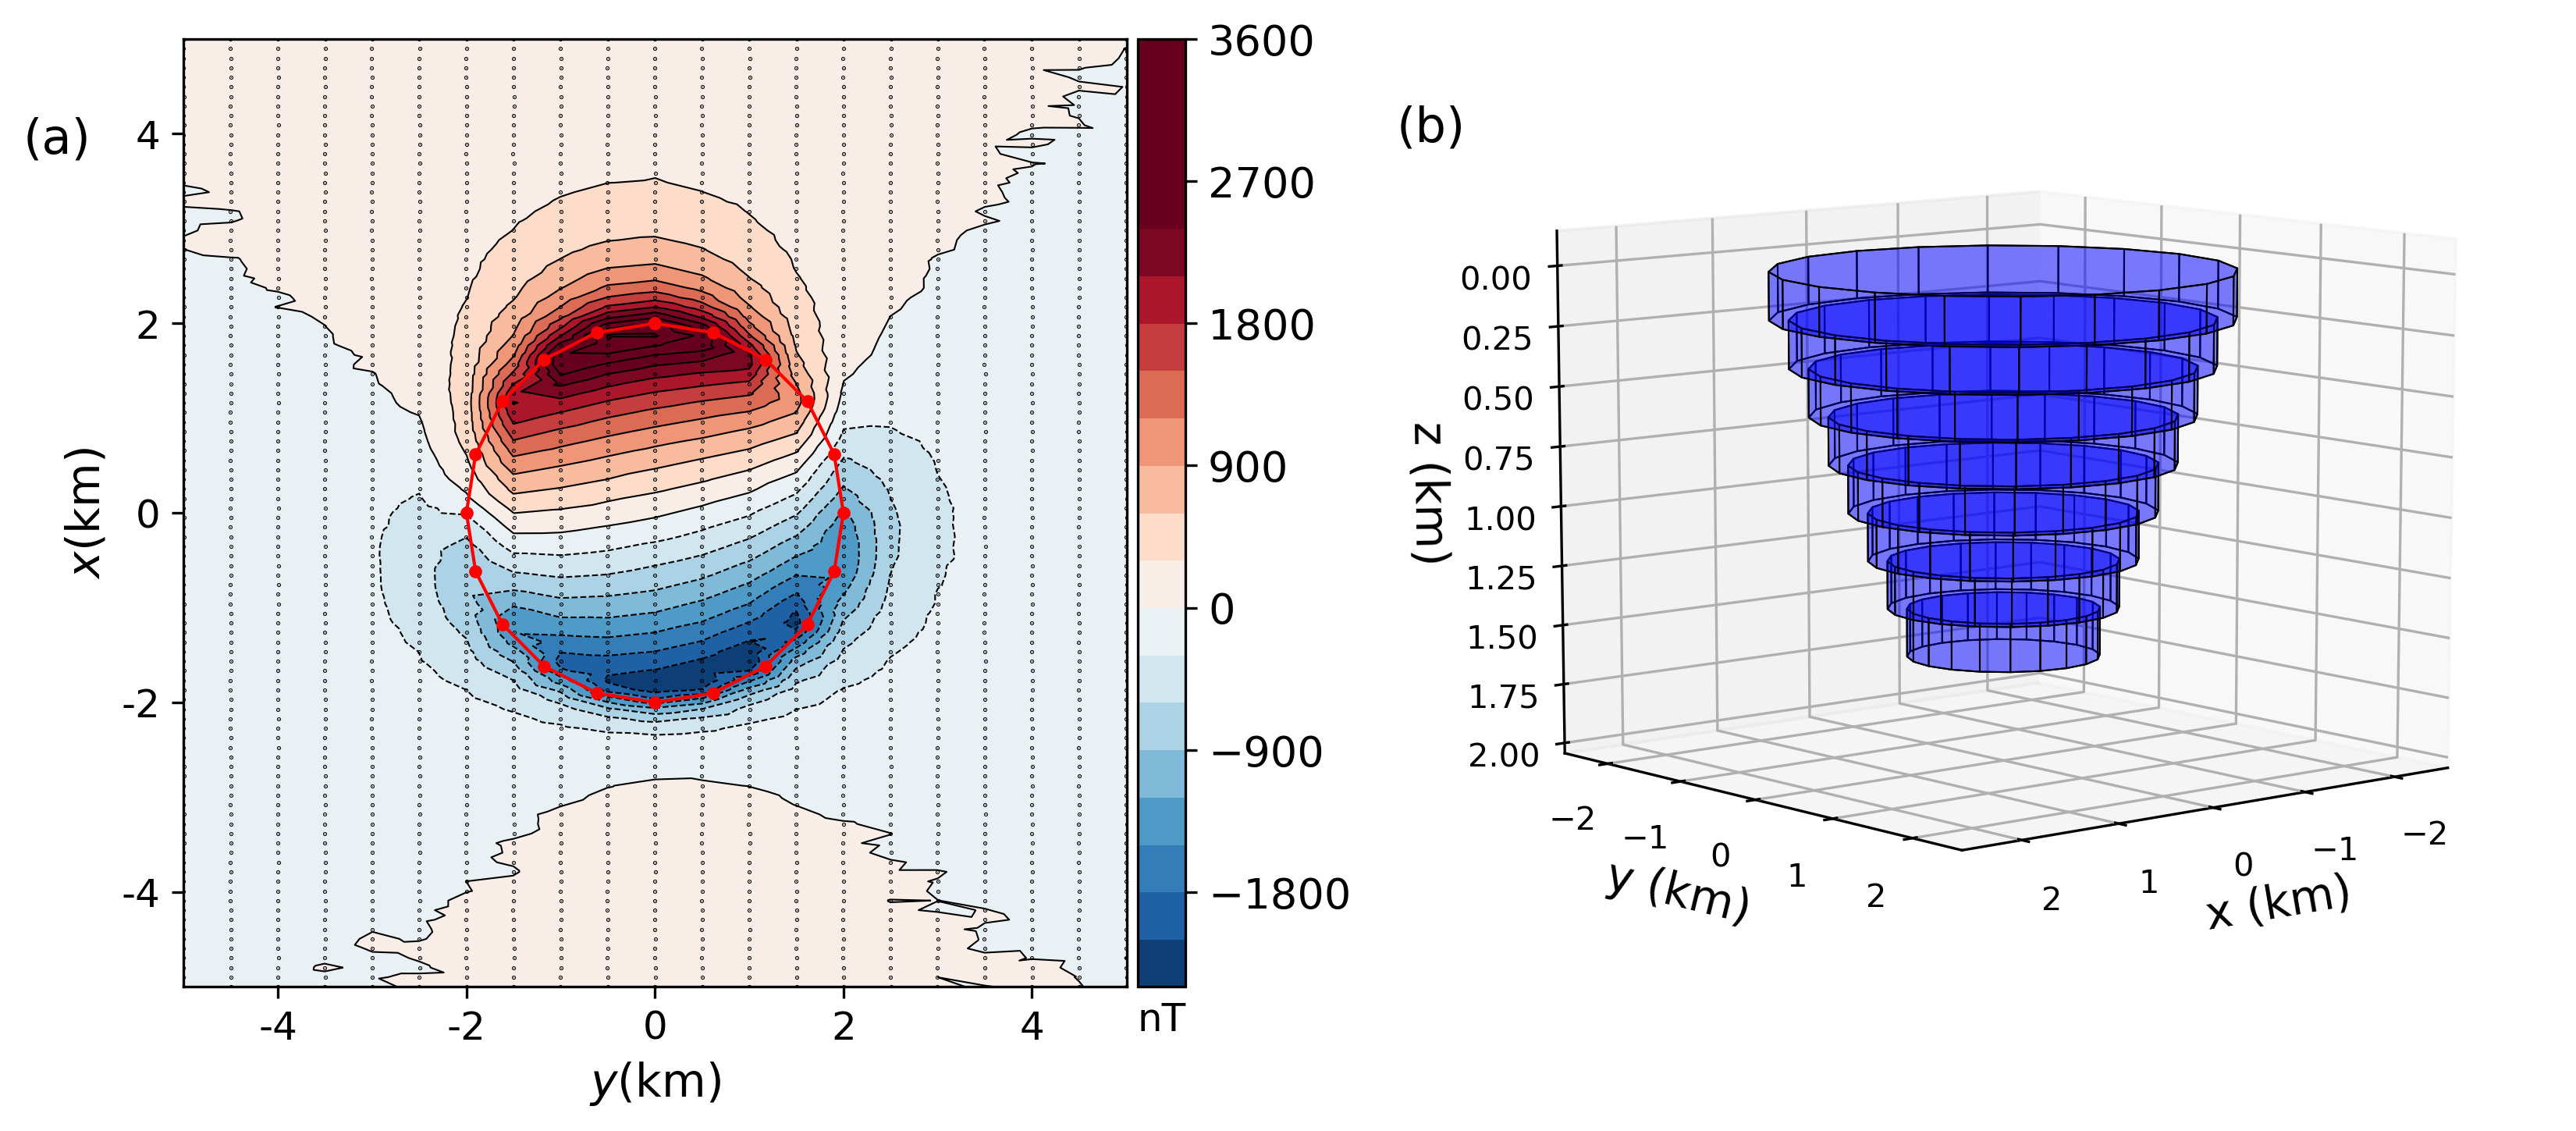
\includegraphics[width=\linewidth]{figures/simple_model_data.png}
    \caption{Simple model simulation. (a) Noise-corrupted total-field anomaly produced by the lopolithic-like body (blue prisms) shown in the panel (b). The black dots represent the observation points. The red circle represents the horizontal projection 
    of the initial approximation $\hat{\mathbf{p}}_{(0)}$
    (red prisms in Fig. \ref{fig:simple_results}b).
    (b) Perspective view of the simple model (lopolithic intrusion) represented by the blue prisms. 
    (c) Discrete map of the goal function $\Gamma(\mathbf{p}, m_0, z_0)$ (Eq.
    \ref{eq:gamma}) produced by the estimates $\hat{\mathbf{p}}_{(f)}$ obtained with
    a $6 \times 6$ grid of tentative values for depth to the top $z_0$ and
    total-magnetization intensity $m_0$.
    The red triangle pinpoint the true and retrieved 	   
    values of $m_0$  and $z_0$. (d) RTP anomaly of the total-field anomaly shown in 
    Fig. \ref{fig:simple_model}a.
}
    \label{fig:simple_model}
\end{figure}

\begin{figure}
	\centering
	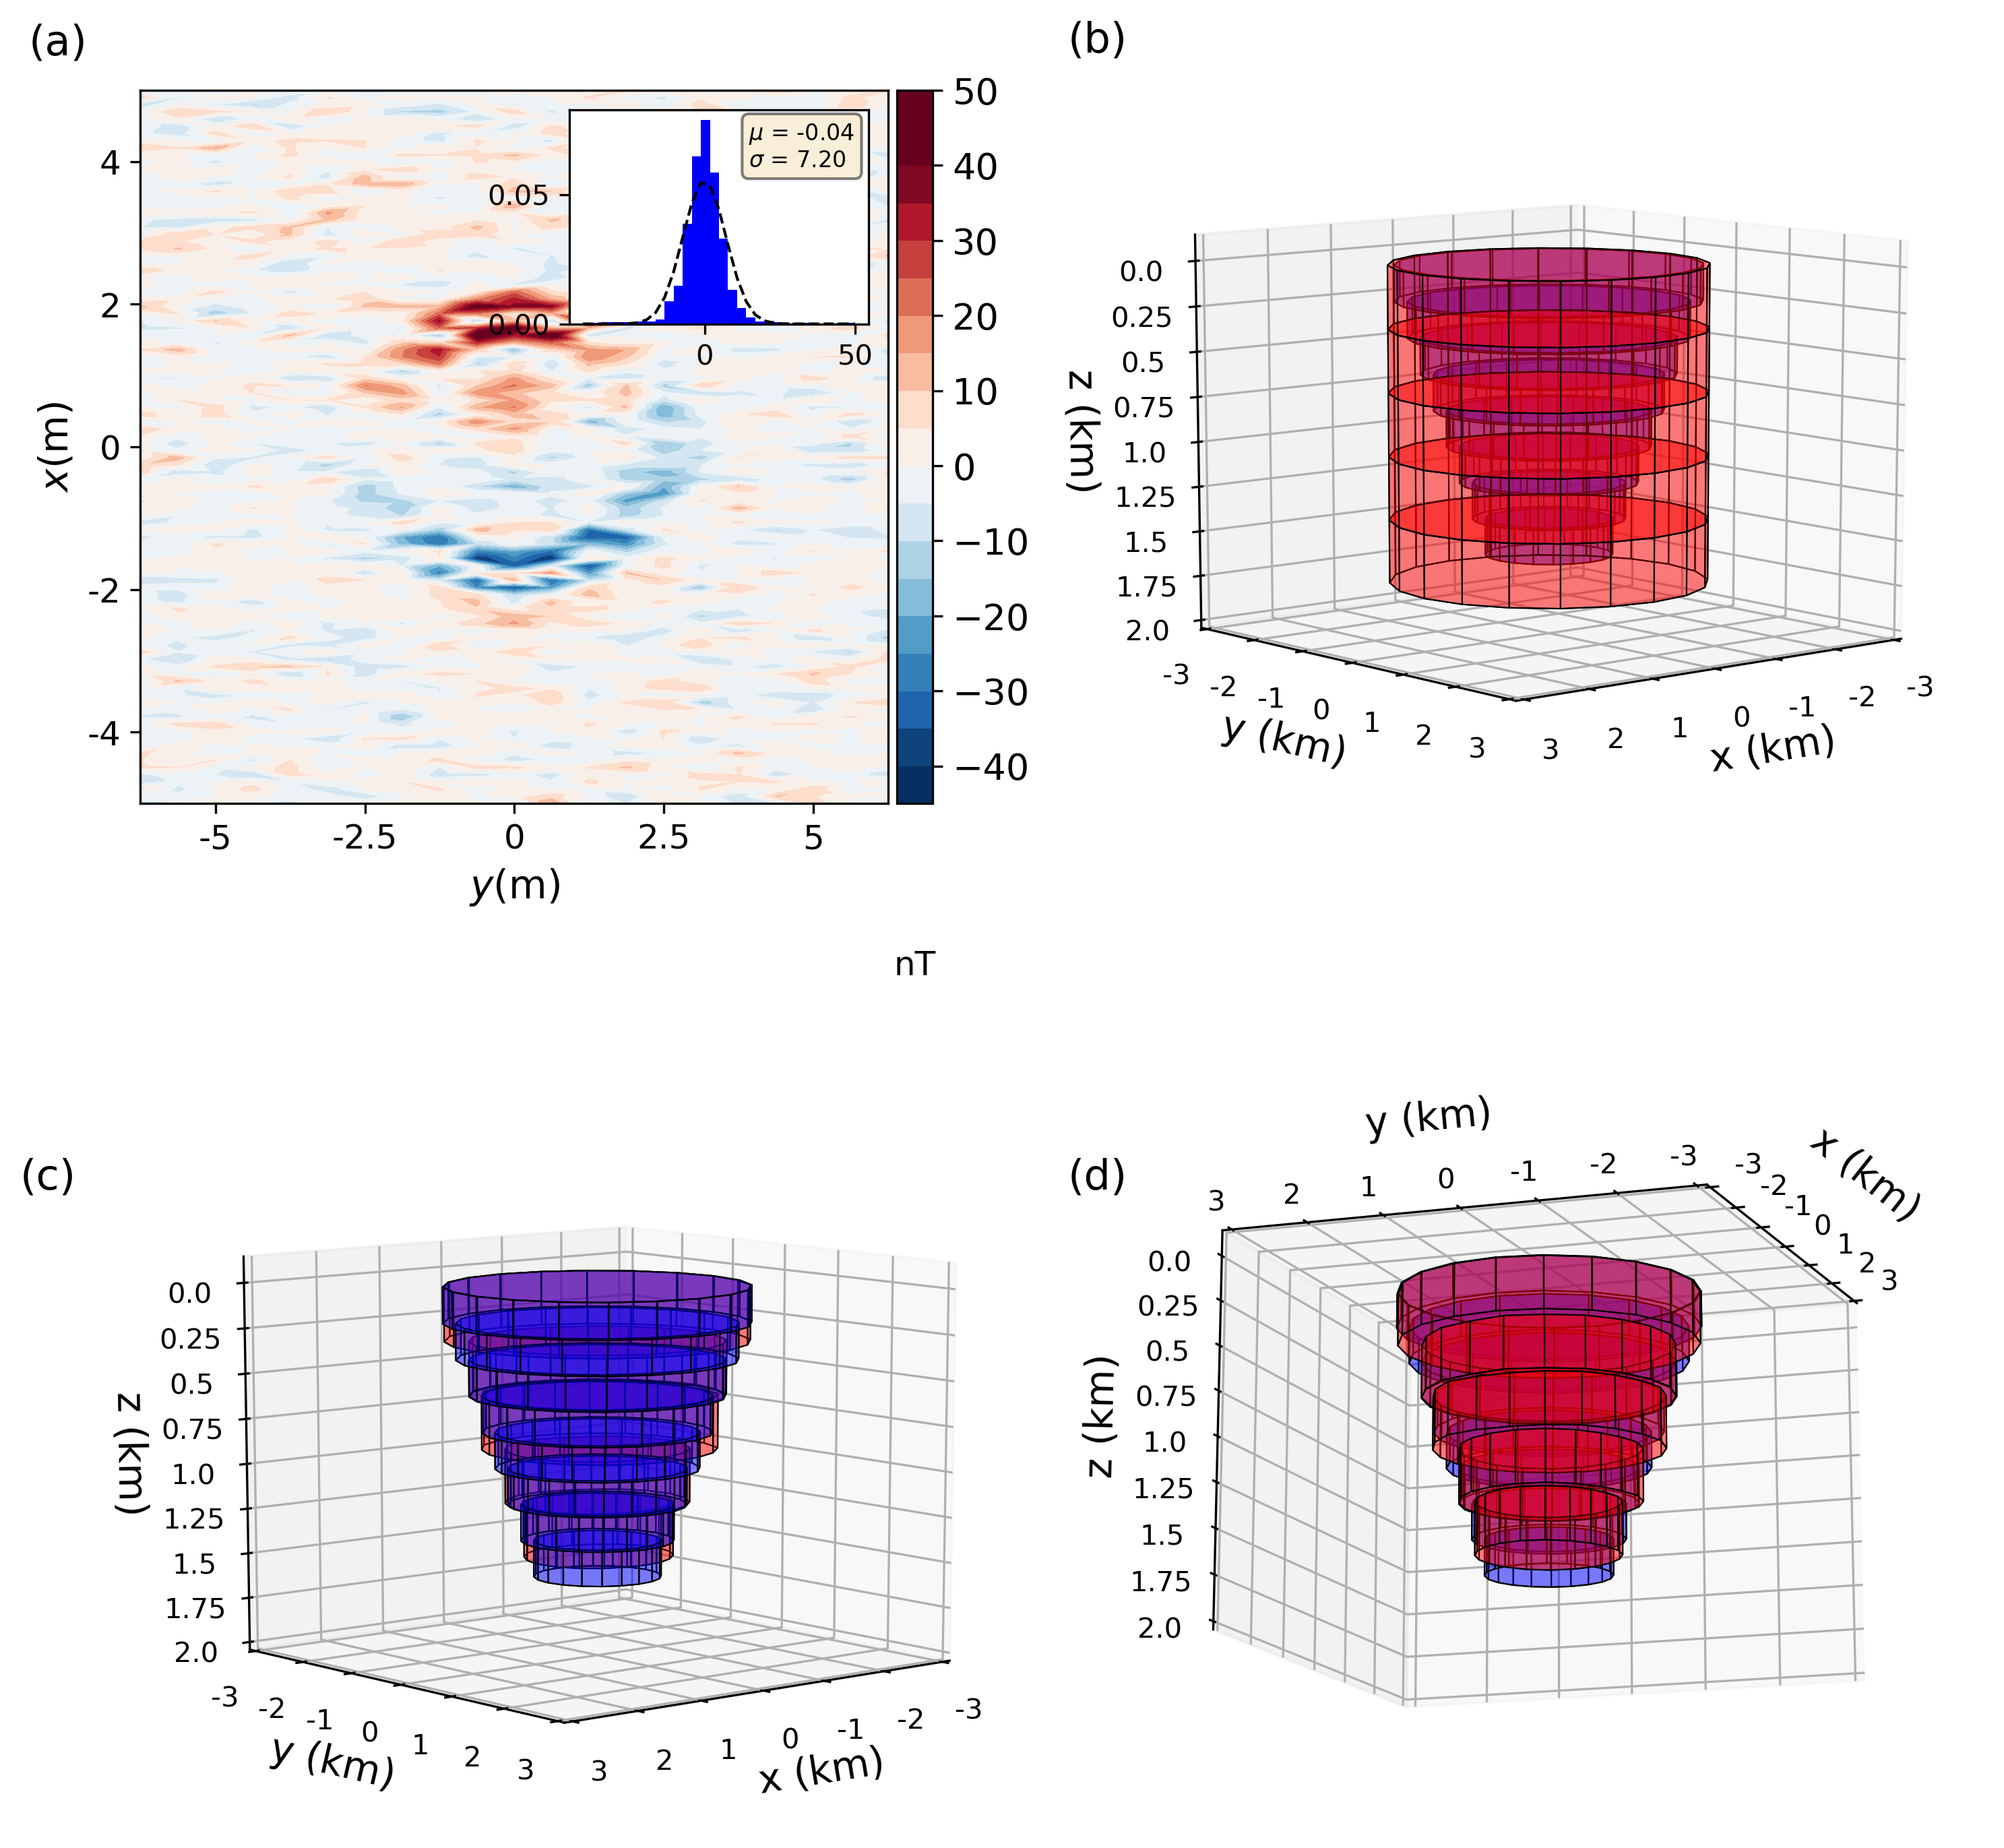
\includegraphics[width=\linewidth]{figures/simple_results.png}
	\caption{Simple model simulation. (a) Residuals between the  noise-corrupted data (Fig. \ref{fig:simple_model}a) and the predicted data (not shown) produced by the estimated model (red prisms shown in the panels (c) and (d)). The inset shows the histogram of the residuals and the Gaussian curve (dashed line) has mean and standard deviation equal to $\mu = -0.04$ nT and $\sigma=7.21$ nT, respectively. (b) Perspective views of the initial approximation (red prisms) and the true model (blue prisms). (c) and (d) Comparison between the estimated source (red prisms) and the true model (blue prisms) in perspective views.}
	\label{fig:simple_results}
\end{figure}

% Application to synthetic data - dipping model

\begin{figure}
    \centering
    \includegraphics[width=\linewidth]{figures/inclined_model_data.png}
    \caption{Dipping model simulation. (a) Noise-corrupted total-field anomaly produced by the dipping model (blue prisms shown in the panels (c) and (d)). The black dots represent the observation points. The red circle represents the horizontal projection 
   	of the initial approximation $\hat{\mathbf{p}}_{(0)}$ 
   	(red prisms in Fig. \ref{fig:dipping_results}). The blue polygon is the horizontal projection of the simulated dipping source.
   	(b) Vertical coordinates of the observations simulating an airborne survey. (c) and (d) Perspective views of the dipping model represented by the blue prisms.
}
    \label{fig:dipping_model}
\end{figure}

\begin{figure}
    \centering
    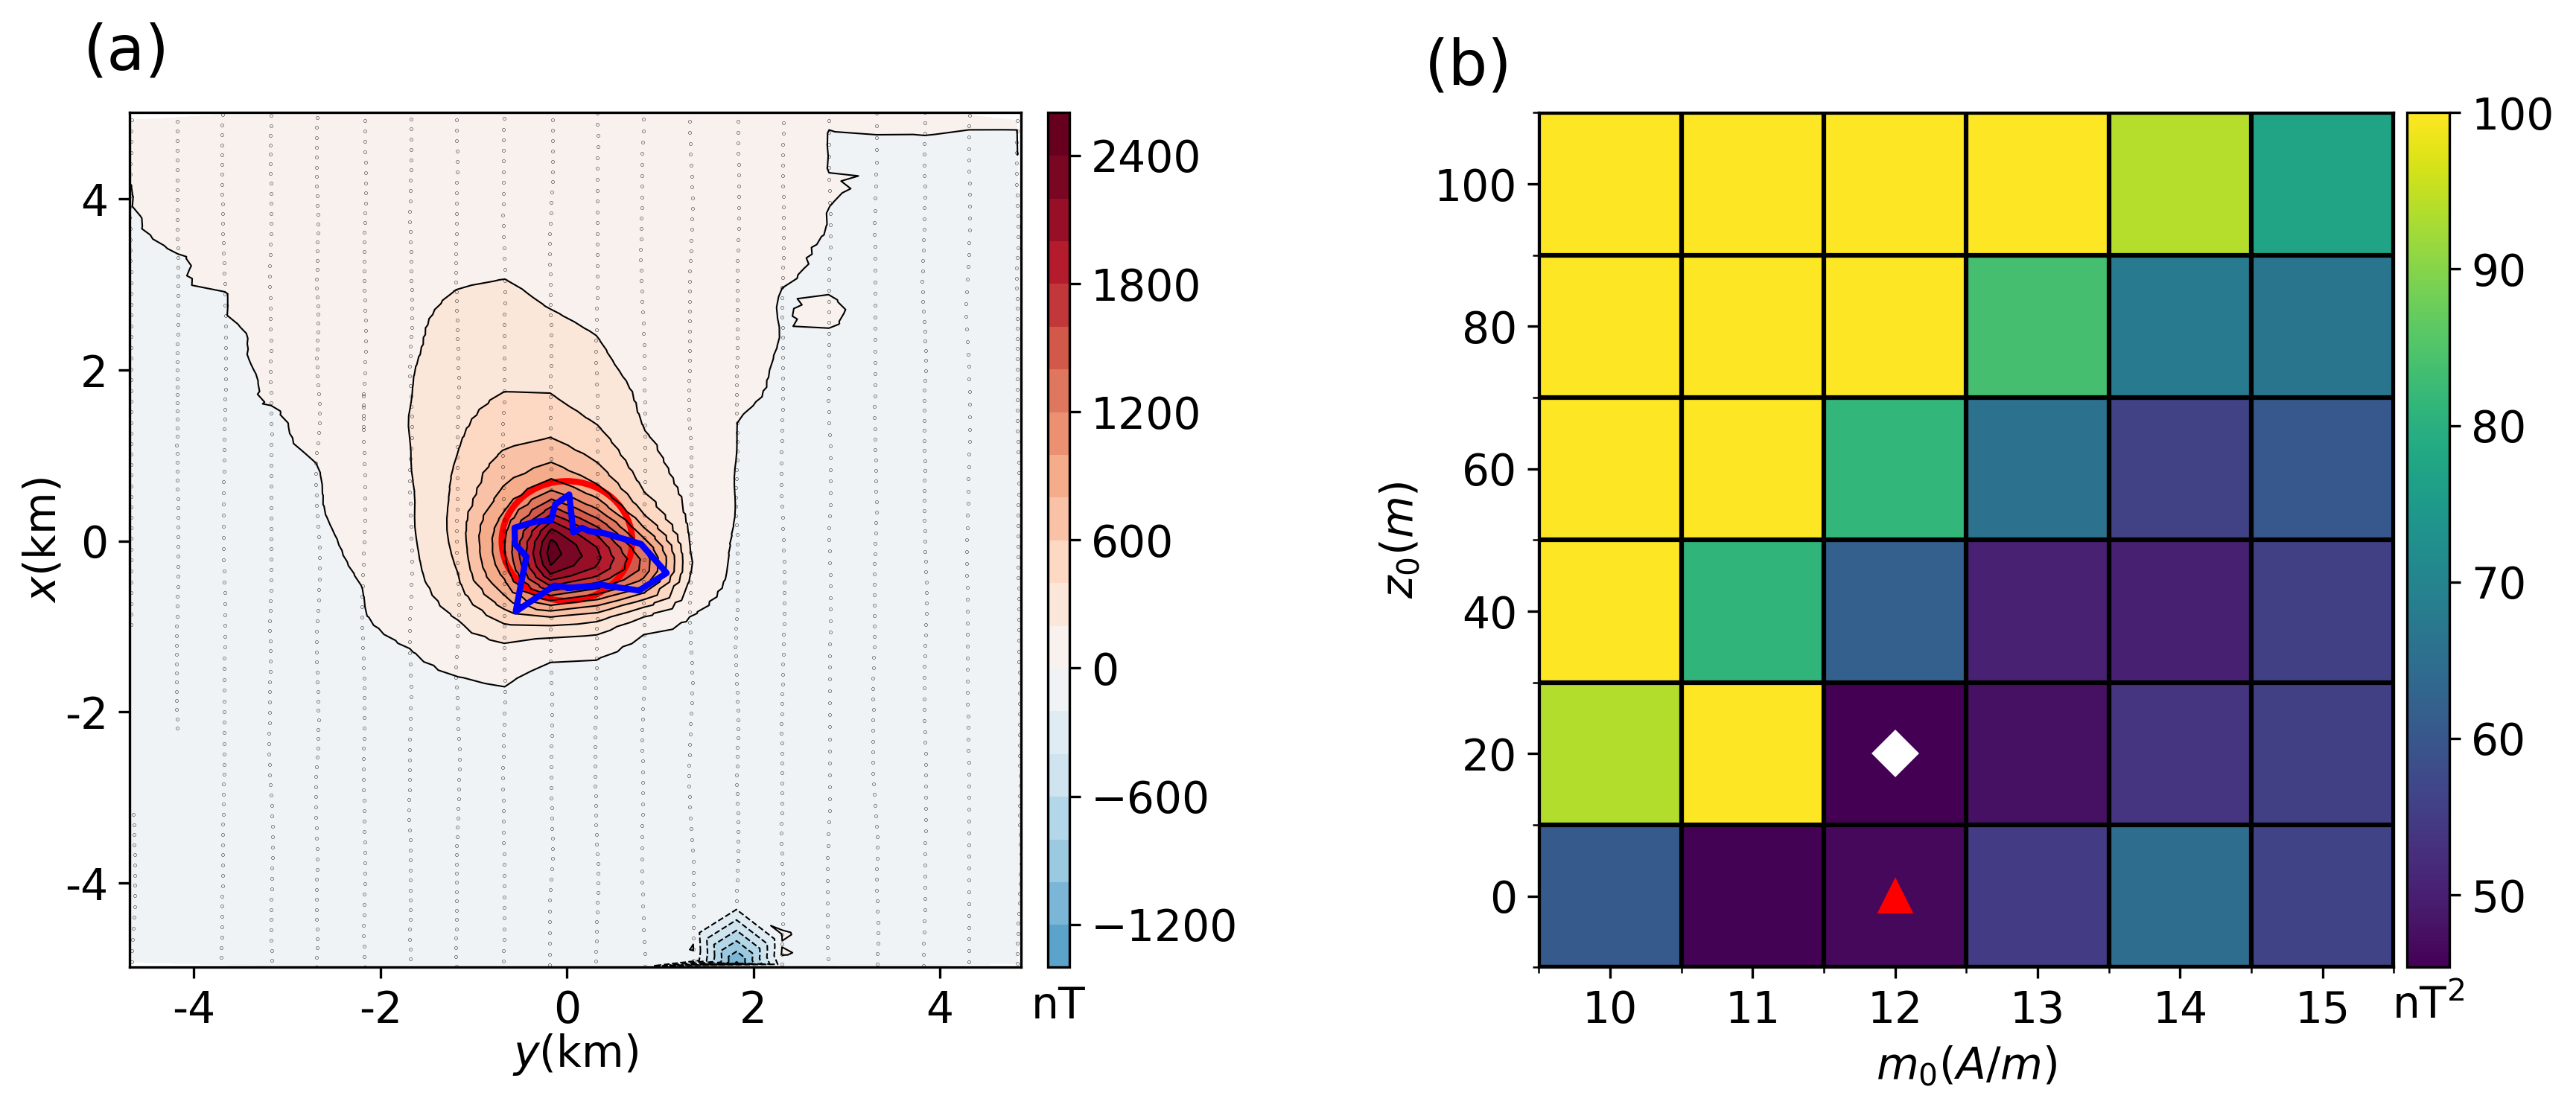
\includegraphics[width=\linewidth]{figures/inclined_rtp.png}
    \caption{Dipping model simulation. (a) RTP anomaly of the total-field anomaly
    shown in Fig. \ref{fig:dipping_model}(a). 
	The red circle and the blue polygon represent the horizontal projections of
	the initial approximation $\hat{\mathbf{p}}_{(0)}$ and  the simulated dipping
	source, respectively.
	(b) Discrete map of the goal function $\Gamma(\mathbf{p}, m_0, z_0)$ (Eq.
	\ref{eq:gamma}) produced by the estimates $\hat{\mathbf{p}}_{(f)}$ obtained with
	a $6 \times 6$ grid of tentative values for depth to the top $z_0$ and
	total-magnetization intensity $m_0$.
	The red triangle  and white diamond pinpoint, respectively, the true and
	retrieved values of $m_0$  and $z_0$.     
}
    \label{fig:dipping_rtp}
\end{figure}


\begin{figure}
    \centering
    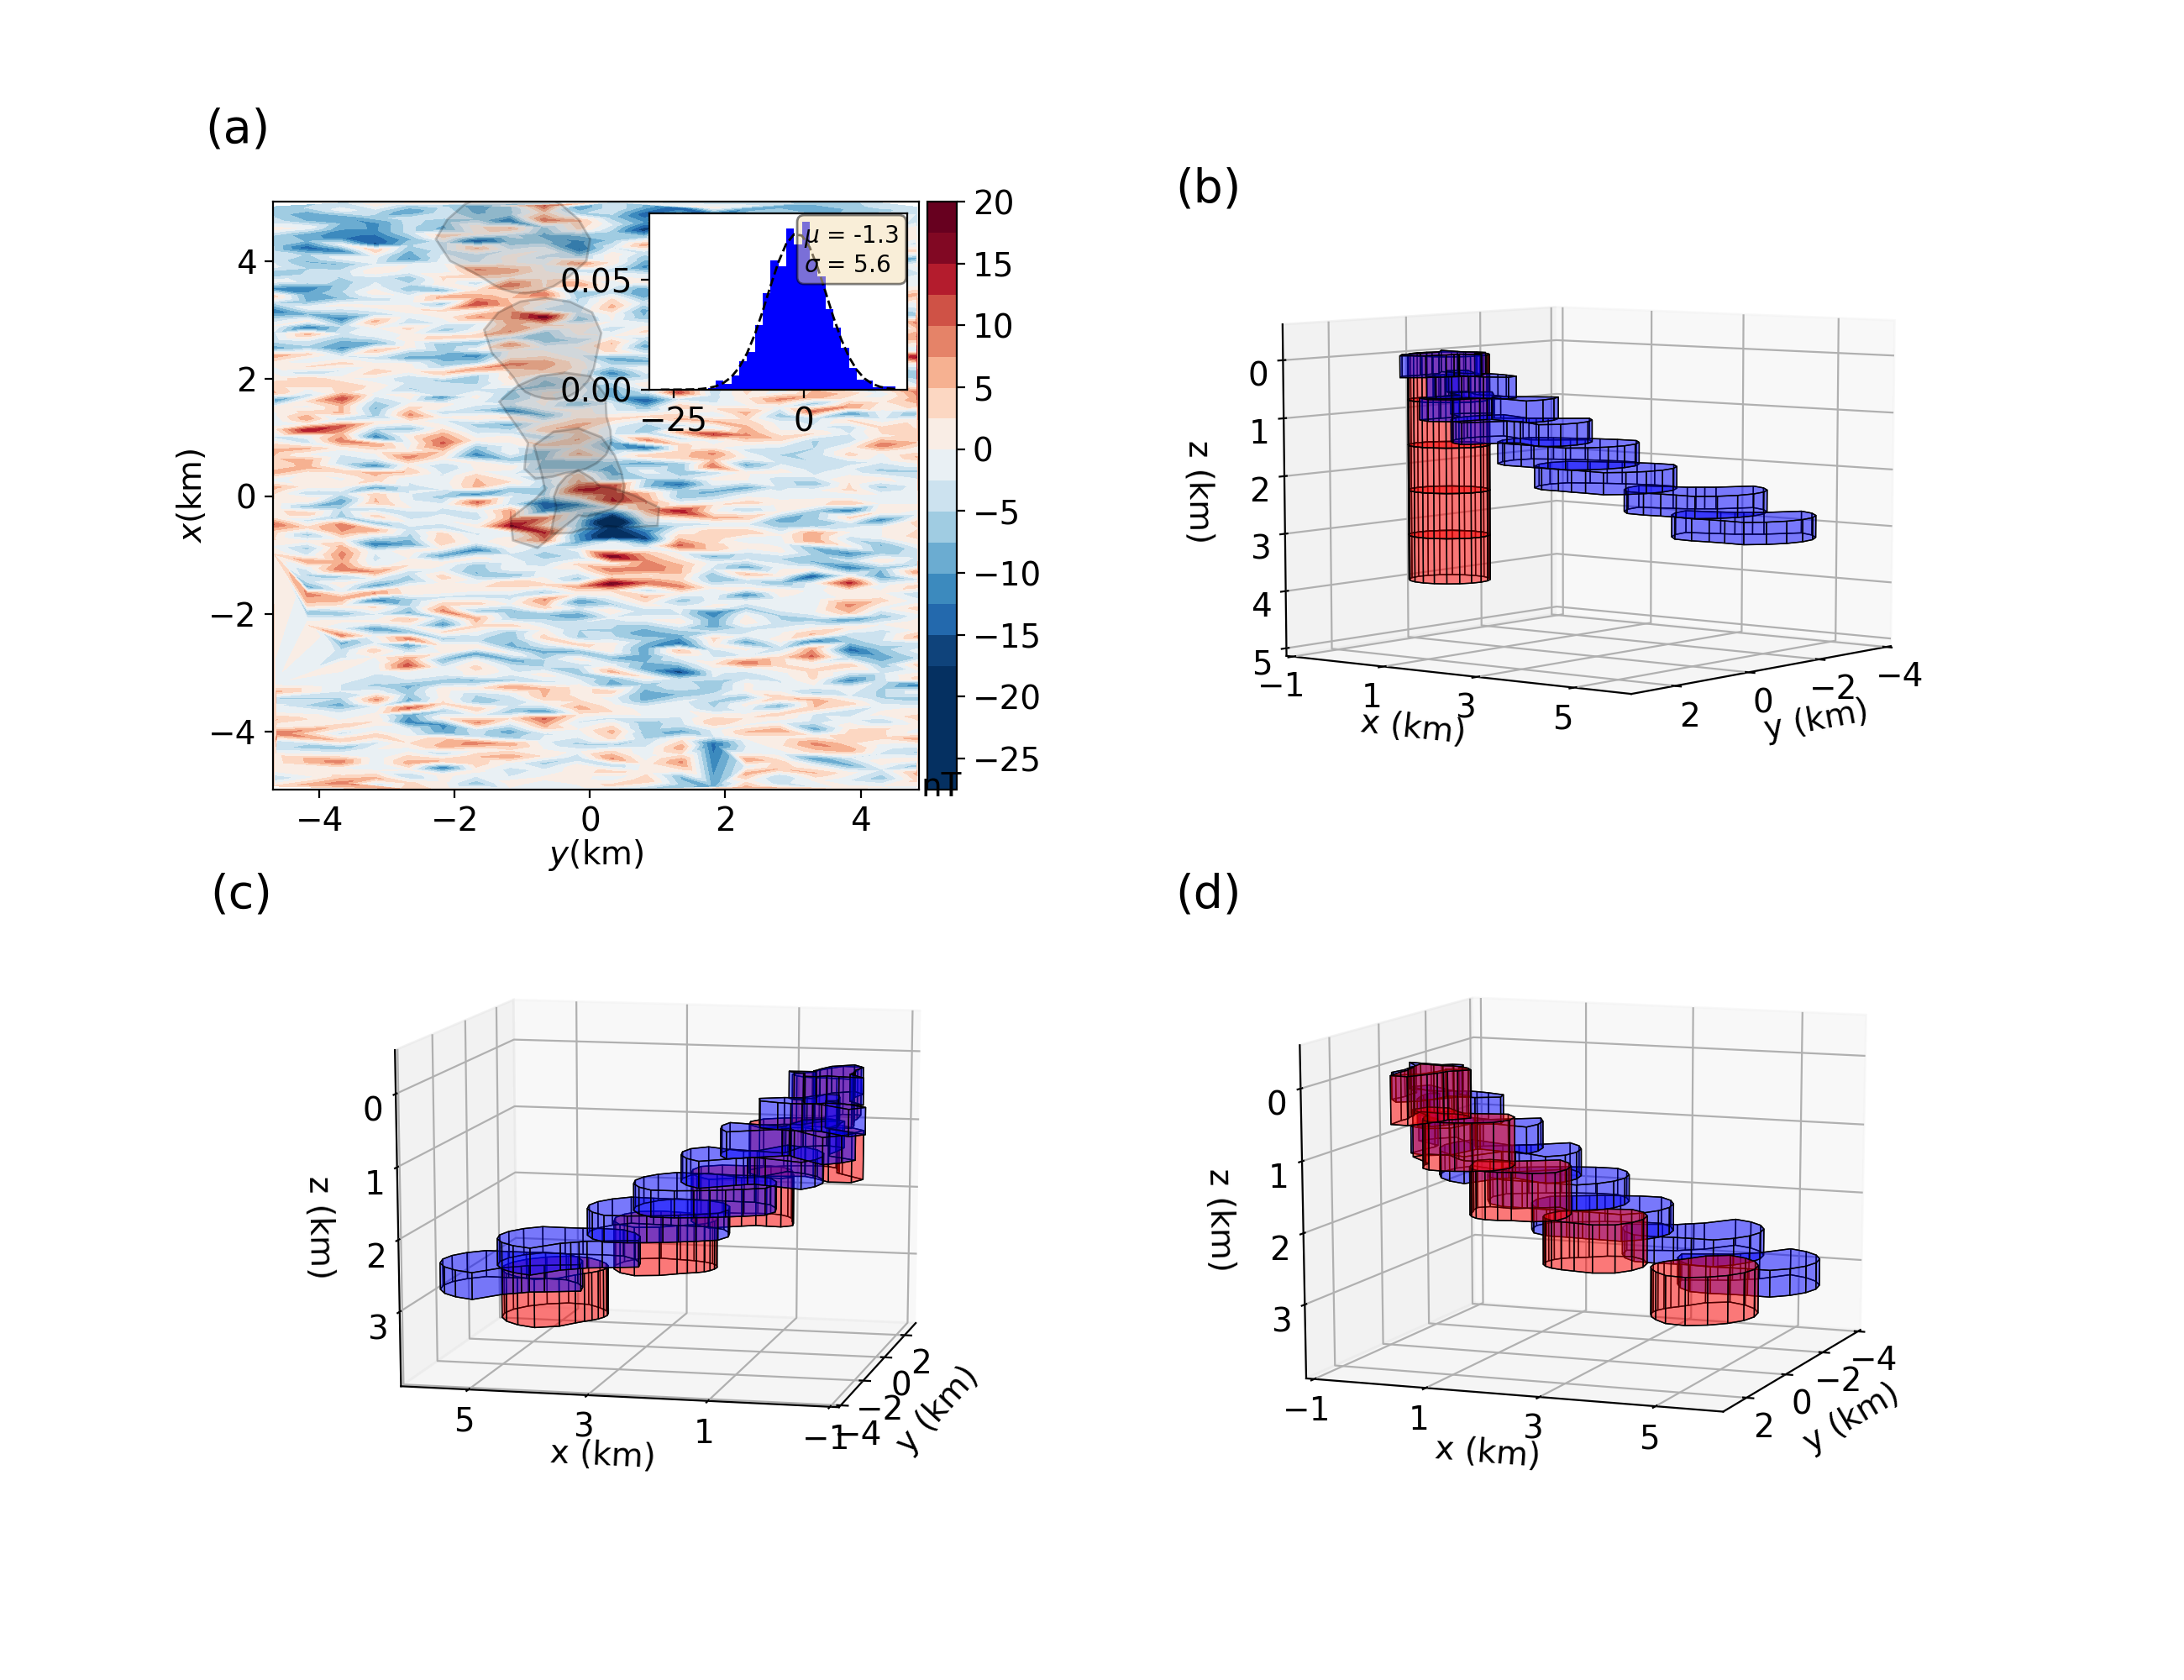
\includegraphics[width=\linewidth]{figures/inclined-l2-solution.png}
    \caption{Dipping model simulation. (a) Residuals between the  noise-corrupted data (Fig. \ref{fig:dipping_model}a) and the predicted data (not shown) produced by the estimated model (red prisms shown in the panels (c) and (d)) using $m_0$  and $z_0$ pinpointed by the white diamond in Fig. \ref{fig:dipping_rtp}b. The inset shows the histogram of the residuals and the Gaussian curve (dashed line) has mean and standard deviation equal 
    to $\mu = 1.3$ nT and $\sigma=5.6$ nT, respectively. 
    The gray polygons are the horizontal projections of the estimated source (red prisms in panels (c) and (d)).
     (b) Perspective views of the initial approximation (red prisms) and the true model (blue prisms). 
     (c) and (d) Comparison between the estimated source (red prisms) and the true model (blue prisms) in perspective views.     
}
    \label{fig:dipping_results}
\end{figure}


% Application to synthetic data - Dipping model in the presence of a regional field test

\begin{figure}
    \centering
    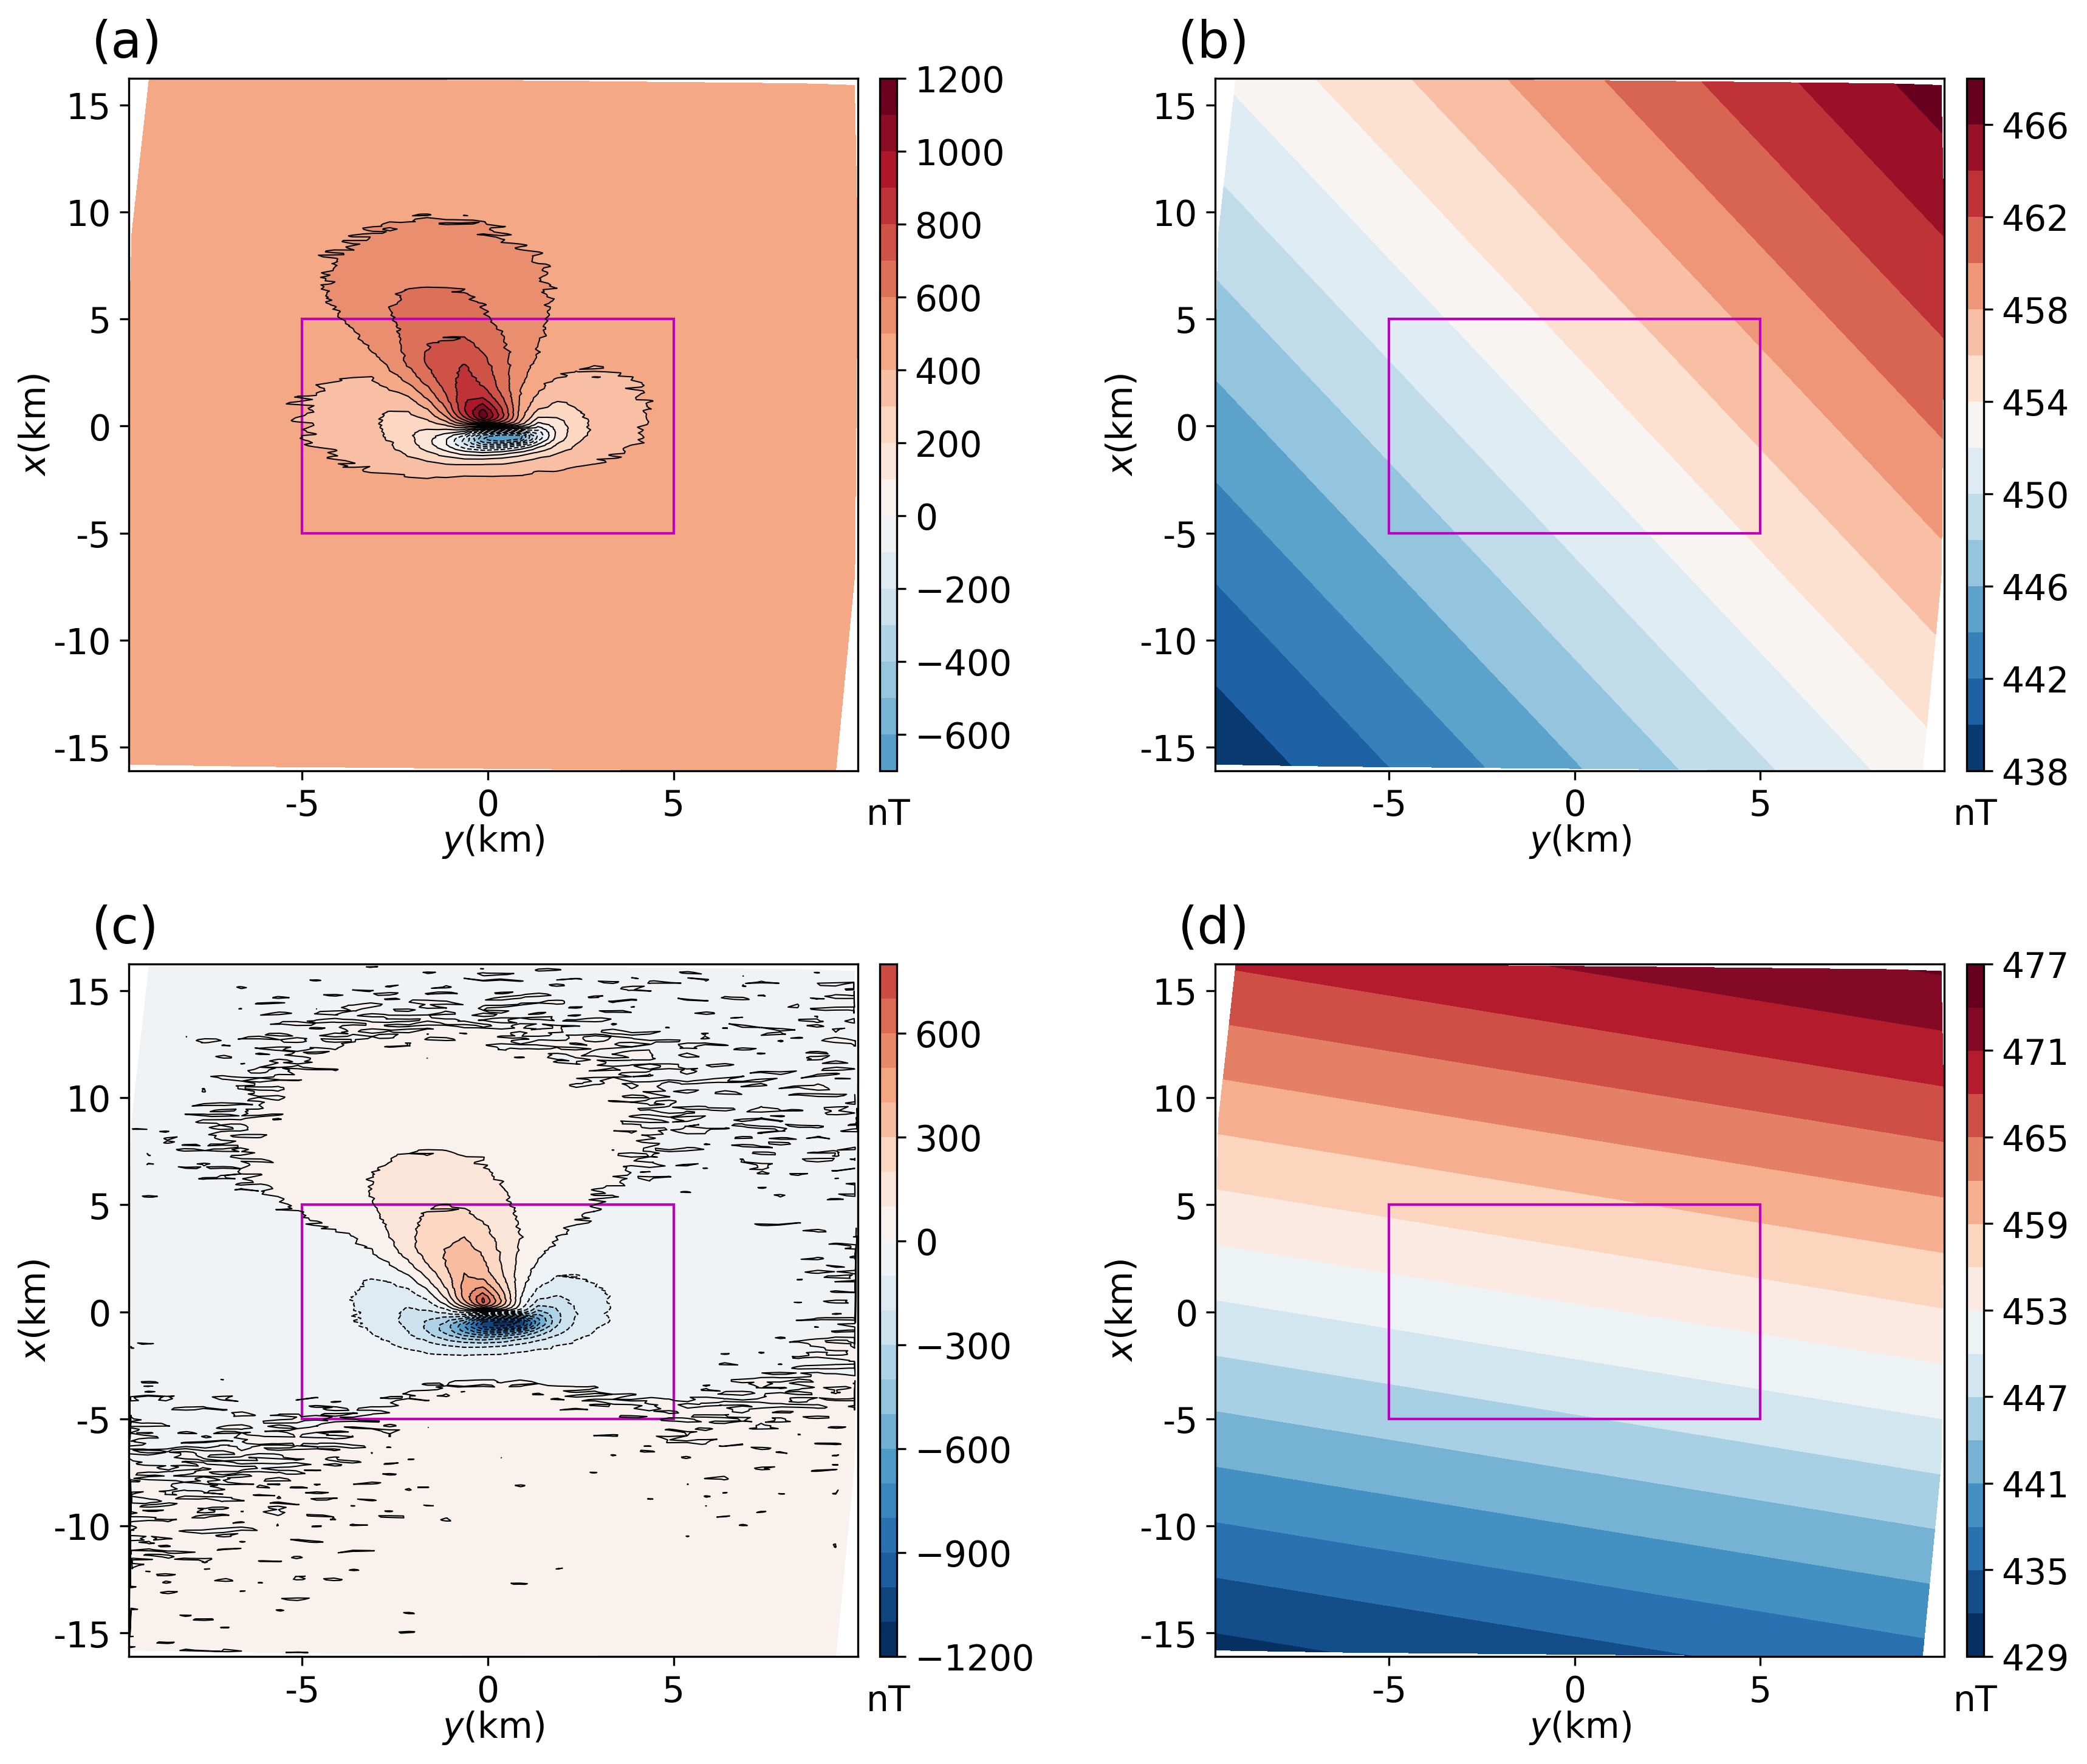
\includegraphics[width=\linewidth]{figures/regional-data-large.png}
    \caption{Dipping model with regional field simulation. (a) Noise-corrupted total-field anomaly composed of a simulated residual field (Fig. \ref{fig:dipping_model}a) due to 
dipping model (blue prisms shown in Fig. \ref{fig:dipping_model}c and d) and a regional field (shown in panel (b)). (b) Simulated regional field through a first-order polynomial. 
(c) Residual total-field anomaly after subtracting from the original anomaly (shown in panel (a)) a
regional total-field anomaly (shown in panel (d)) obtained by a least-squares polynomial fitting. 
(d)  Regional total-field anomaly approximated by a least-squares polynomial fitting to the original anomaly (shown in panel (a)). The magenta rectangle delimits the data to be inverted.
}
    \label{fig:dipping_regional_model}
\end{figure}

\begin{figure}
    \centering
    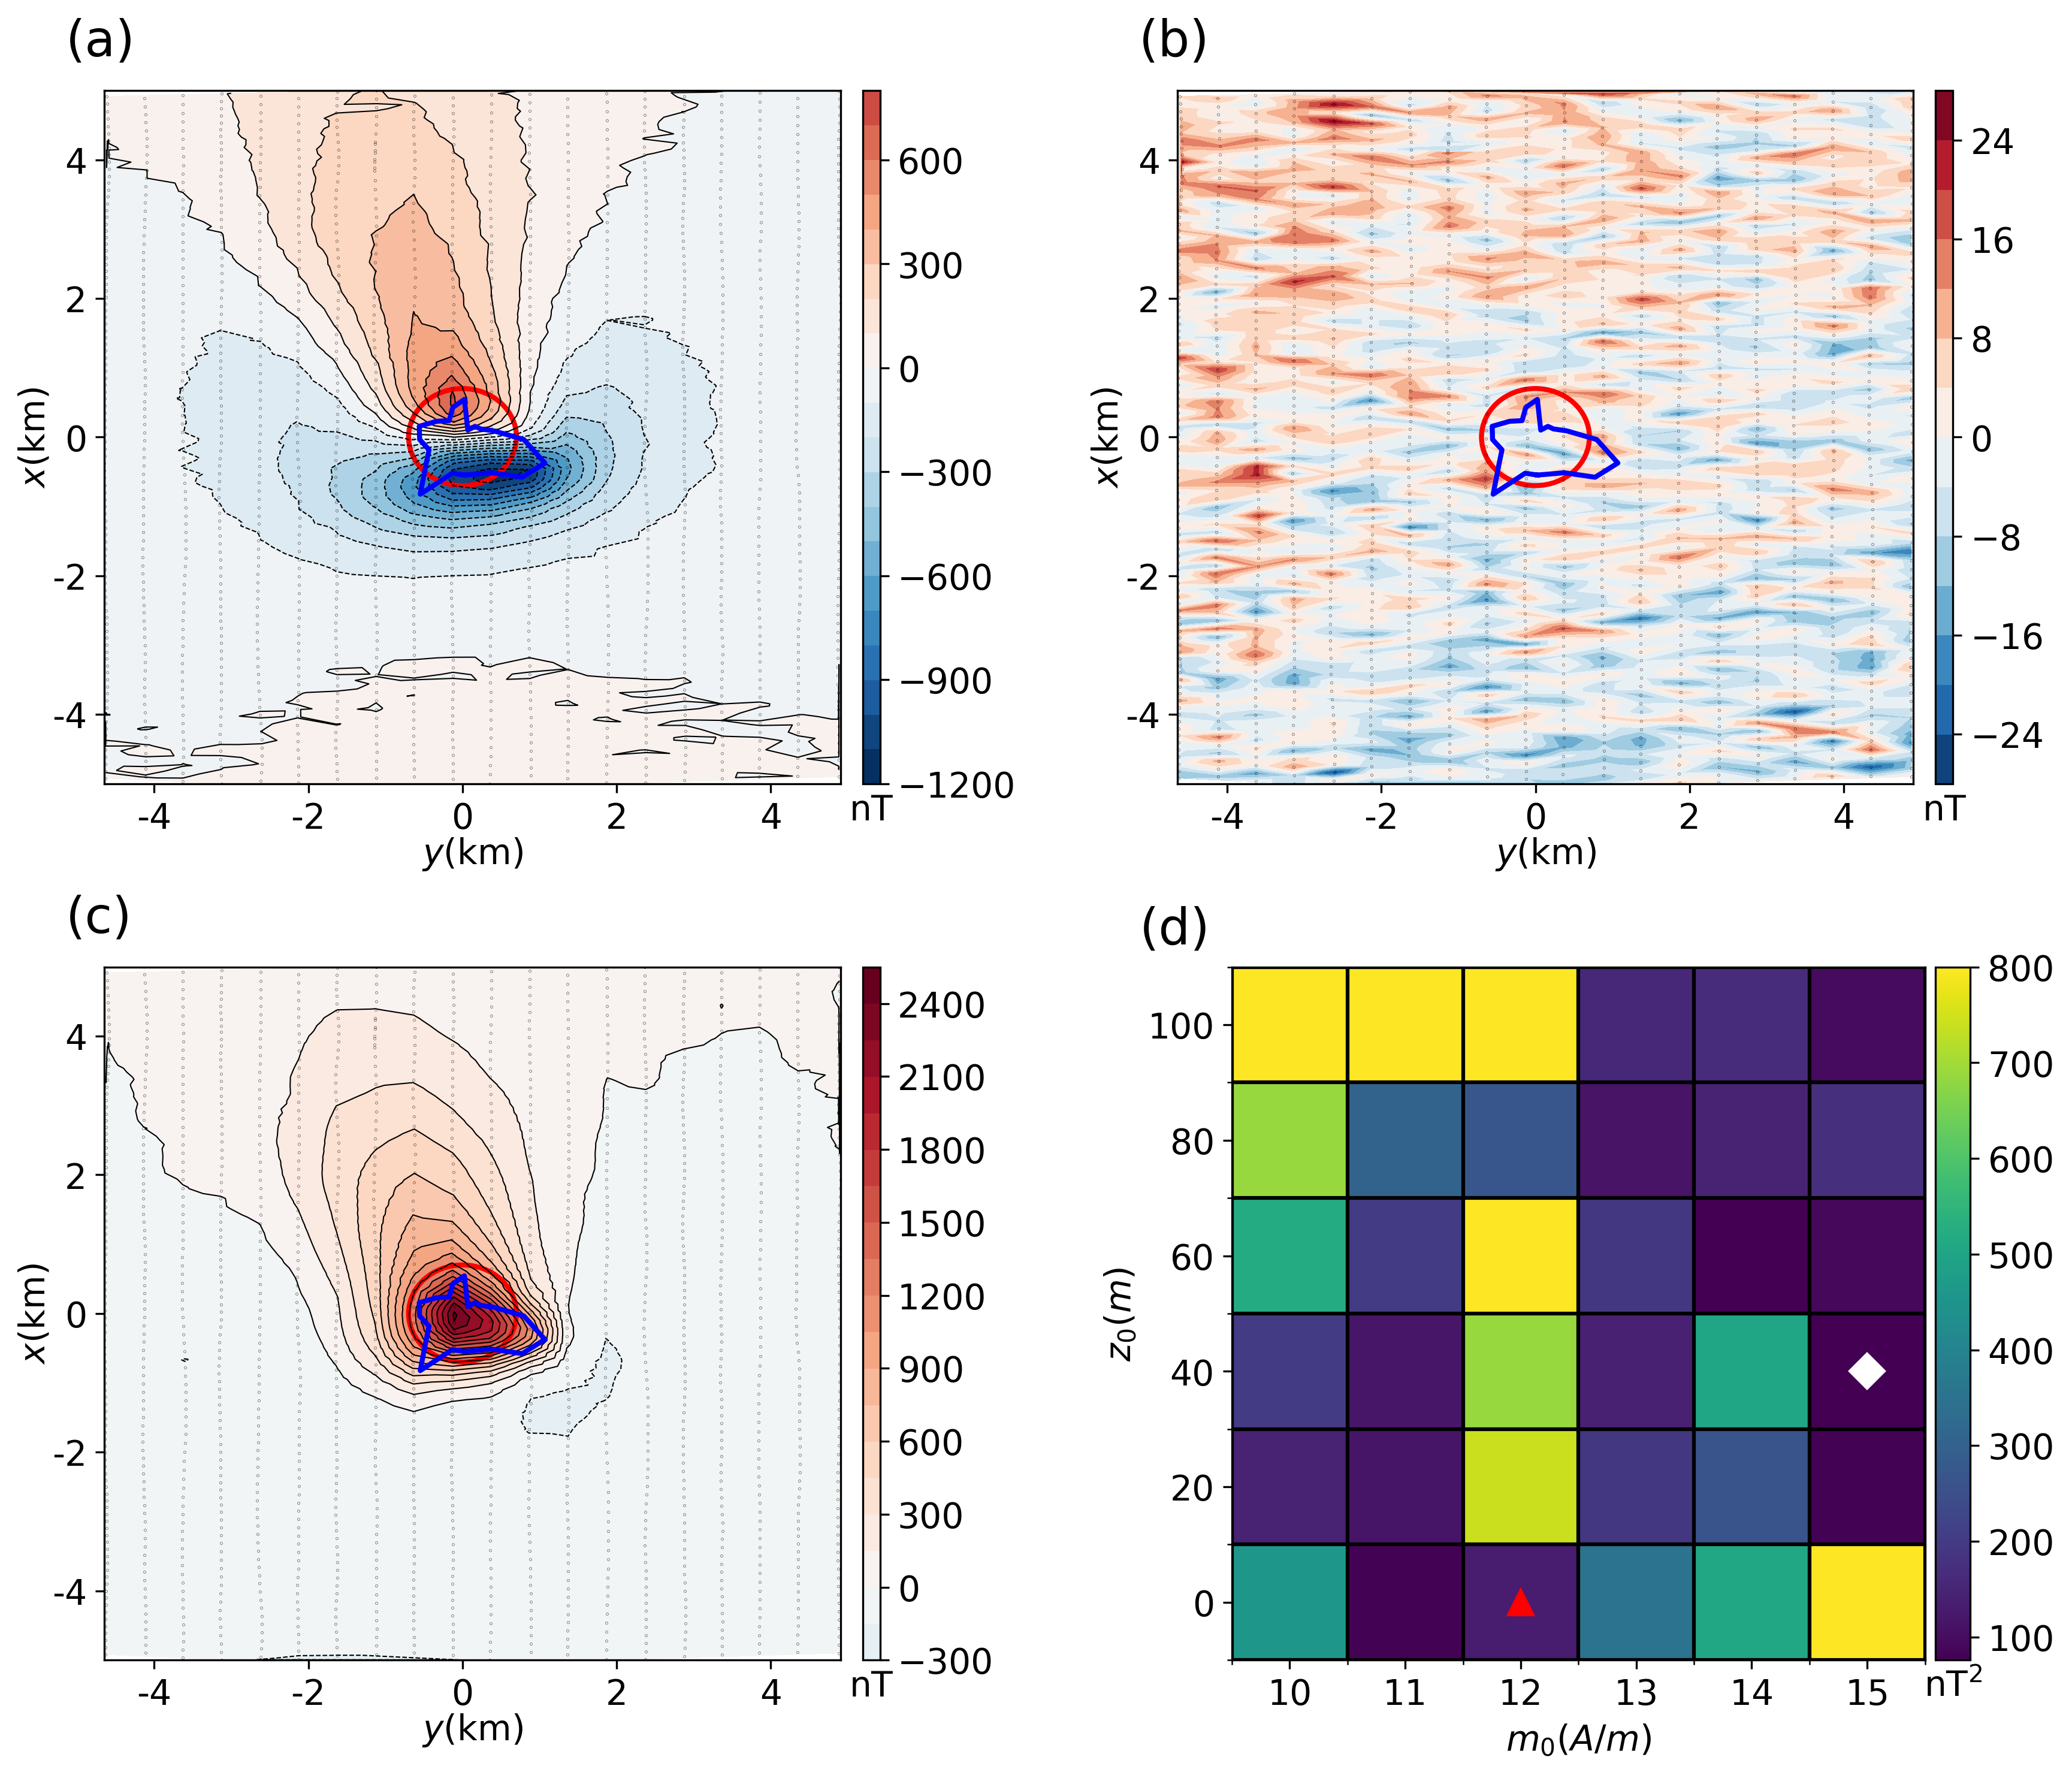
\includegraphics[width=\linewidth]{figures/regional_rtp.png}
    \caption{Dipping model with regional field simulation. (a) Residual total-field
    anomaly to be inverted over the area delimited by the  magenta rectangle 
    in Fig. \ref{fig:dipping_regional_model}(c). 
    (b) Differences between the total-field anomaly produced by the dipping model
    (Fig. \ref{fig:dipping_model}a) and the residual total-field anomaly (shown in
    panel (a)) after a regional-residual separation using a least-squares polynomial
    fitting. 
    (c) RTP anomaly of the  residual total-field anomaly shown in panel (a). 
    (d) Discrete map of the goal function $\Gamma(\mathbf{p}, m_0, z_0)$ (Eq.
    \ref{eq:gamma}) produced by the estimates $\hat{\mathbf{p}}_{(f)}$ obtained with
    a $6 \times 6$ grid of tentative values for depth to the top $z_0$ and
    total-magnetization intensity $m_0$.
    The red triangle  and white diamond pinpoint, respectively, the true and
    retrieved values of $m_0$  and $z_0$.
    In the panels (a)-(c), the red circle and the blue polygon represent the
    horizontal projections of the initial approximation $\hat{\mathbf{p}}_{(0)}$ 
    and the simulated dipping source, respectively.
}
    \label{fig:dipping_regional_rtp}
\end{figure}


\begin{figure}
    \centering
    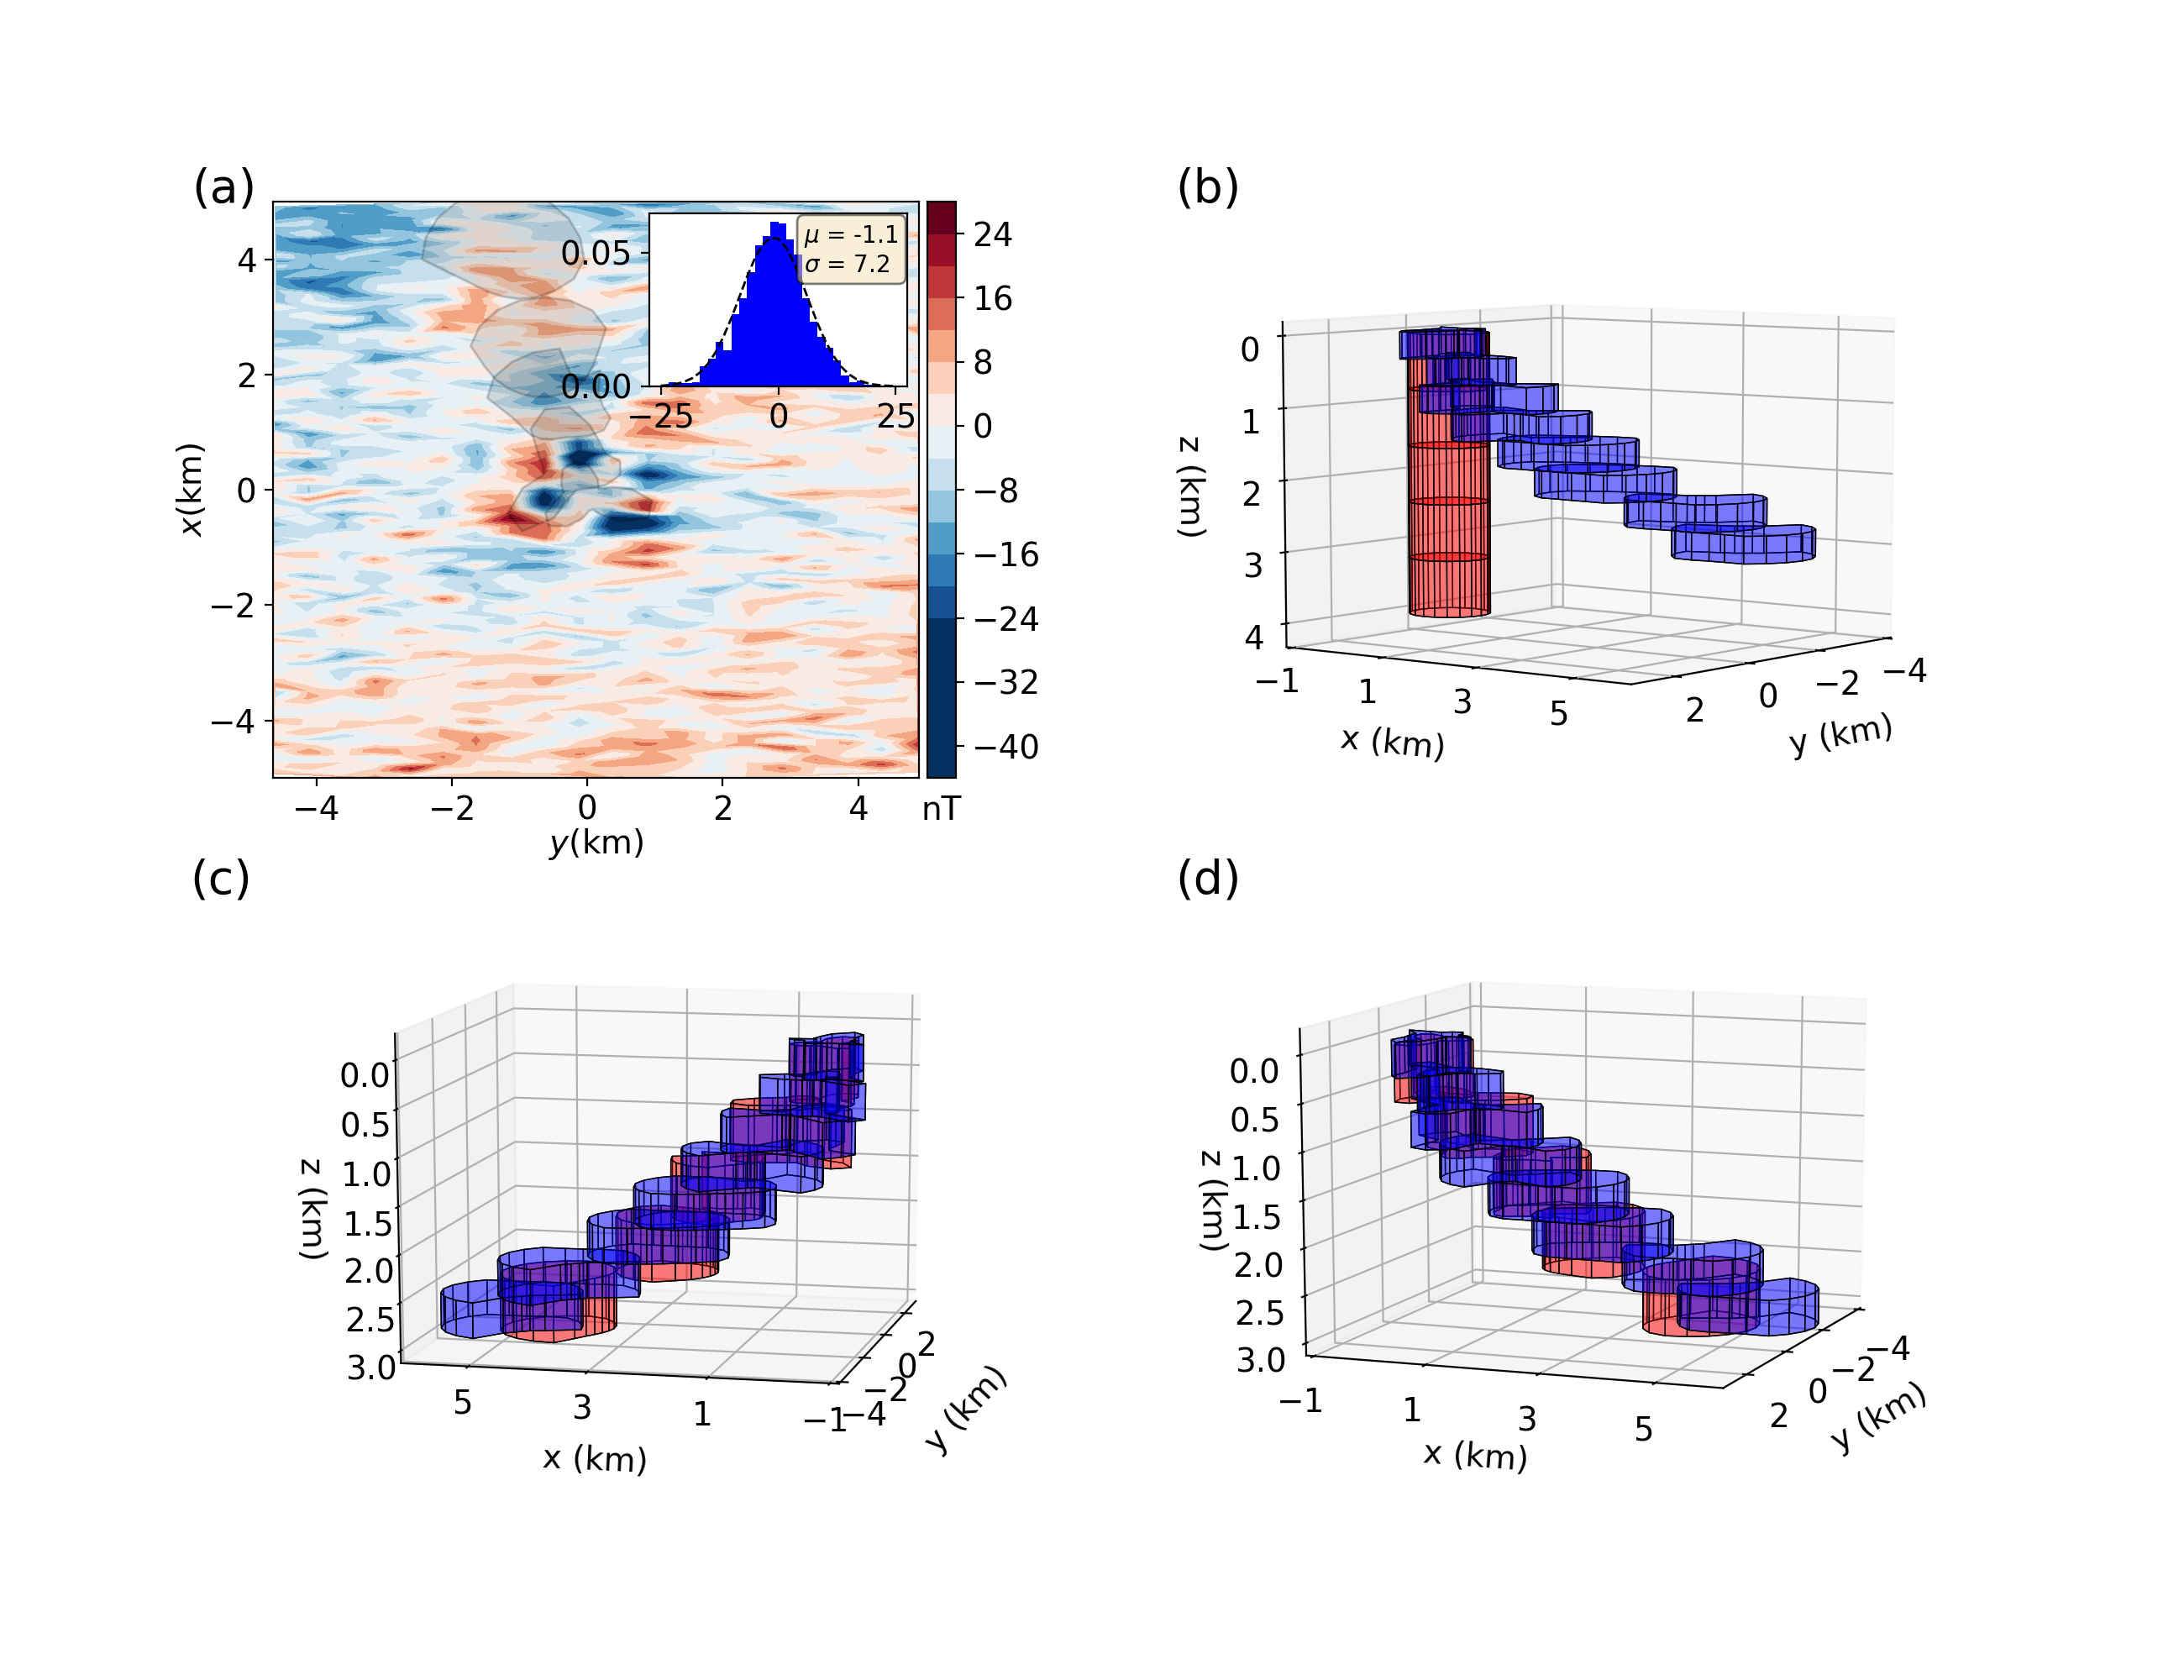
\includegraphics[width=\linewidth]{figures/regional-l2-solution.png}
    \caption{Dipping model with regional field simulation. (a) Residuals between the  noise-corrupted data (Fig. \ref{fig:dipping_regional_rtp}a) and the predicted data (not shown) produced by the estimated model (red prisms shown in the panels (c) and (d)) using 
$m_0$  and $z_0$ pinpointed by the white diamond in Fig. \ref{fig:dipping_regional_rtp}d.
The inset shows the histogram of the residuals and the Gaussian curve (dashed line) has mean and standard deviation equal   to $\mu = -1.1$ nT and $\sigma=7.2$ nT, respectively. 
    The gray polygons are the horizontal projections of the estimated source (red prisms in panels (c) and (d)).
     (b) Perspective views of the initial approximation (red prisms) and the true model (blue prisms). 
     (c) and (d) Comparison between the estimated source (red prisms) and the true model (blue prisms) in perspective views.     
}
    \label{fig:regional-results}
\end{figure}

% Application to synthetic data - complex model

\begin{figure}
    \centering
    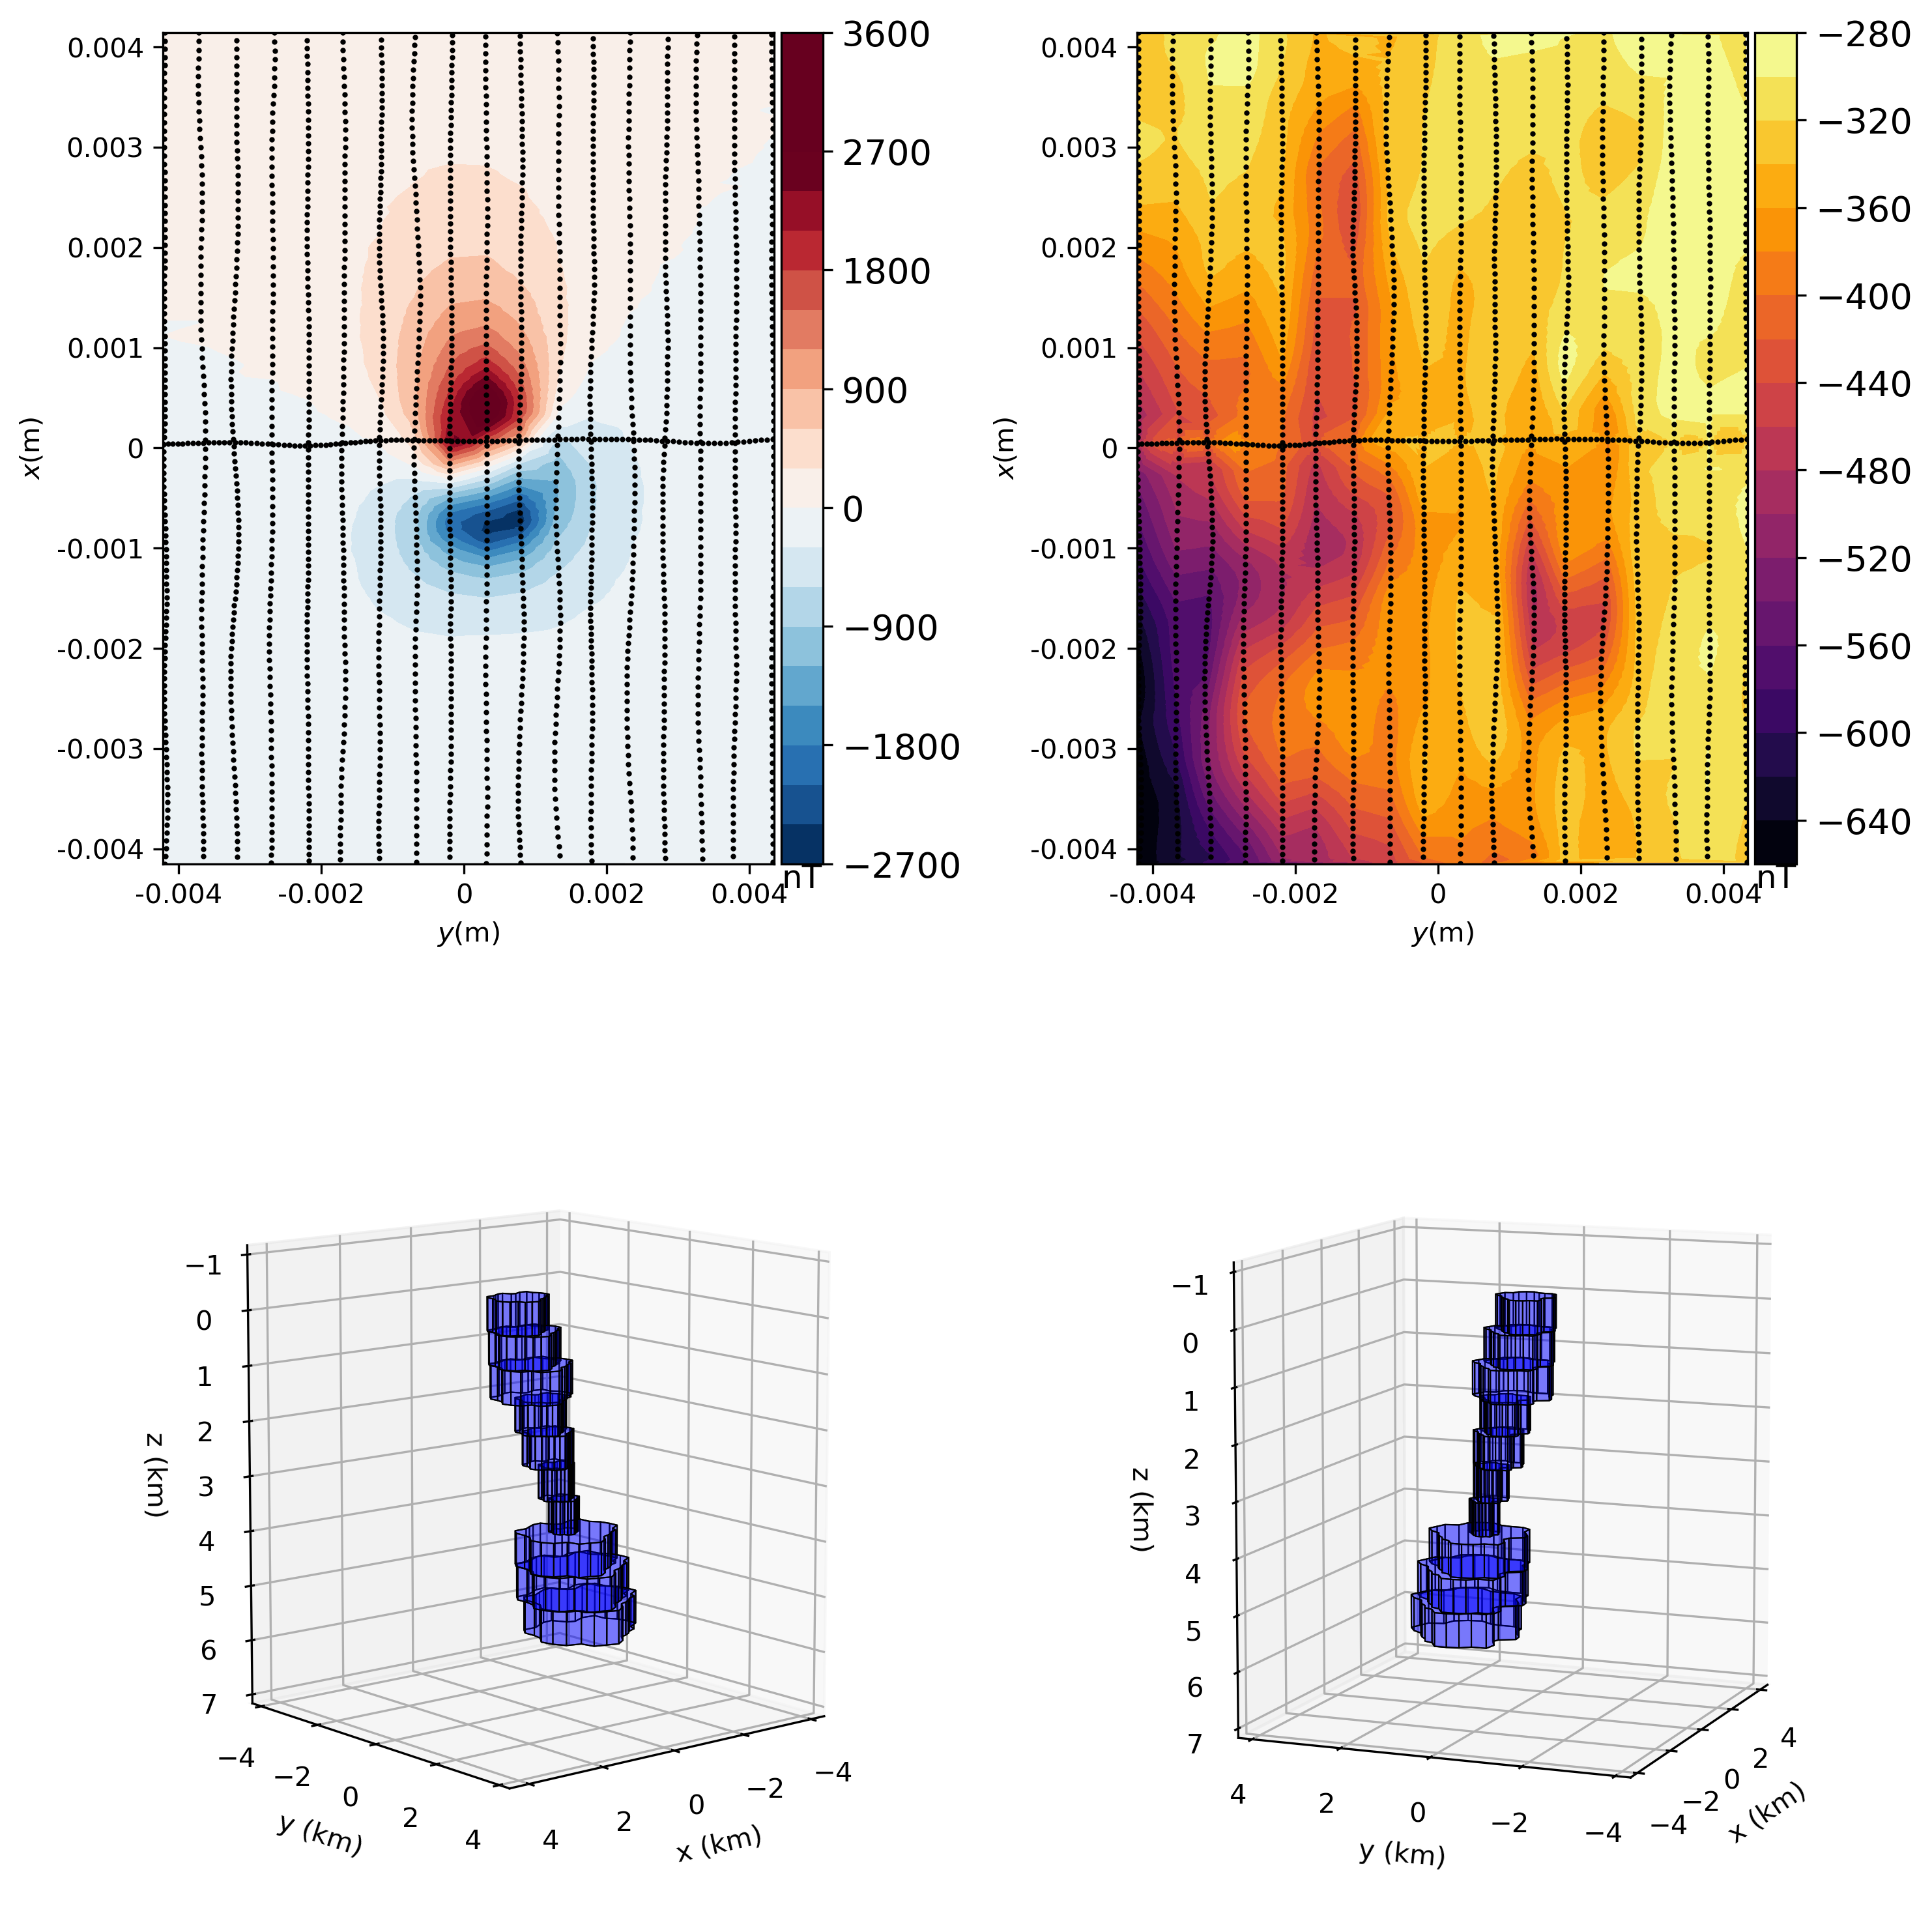
\includegraphics[width=\linewidth]{figures/complex_model_data.png}
    \caption{Complex model simulation. (a) Noise-corrupted total-field anomaly produced by the complex model (blue prisms shown in the panels (c) and (d)). The black dots represent the observation points. The connected red dots represent the horizontal projection 
   	of the initial approximation $\hat{\mathbf{p}}_{(0)}$ 
   	(red prisms in Fig. \ref{fig:complex_result}b). (b) Vertical coordinates of the observations simulating an airborne survey. (c) and (d) Perspective views of the complex model represented by the blue prisms.
}
    \label{fig:complex_model}
\end{figure}

\begin{figure}
    \centering
    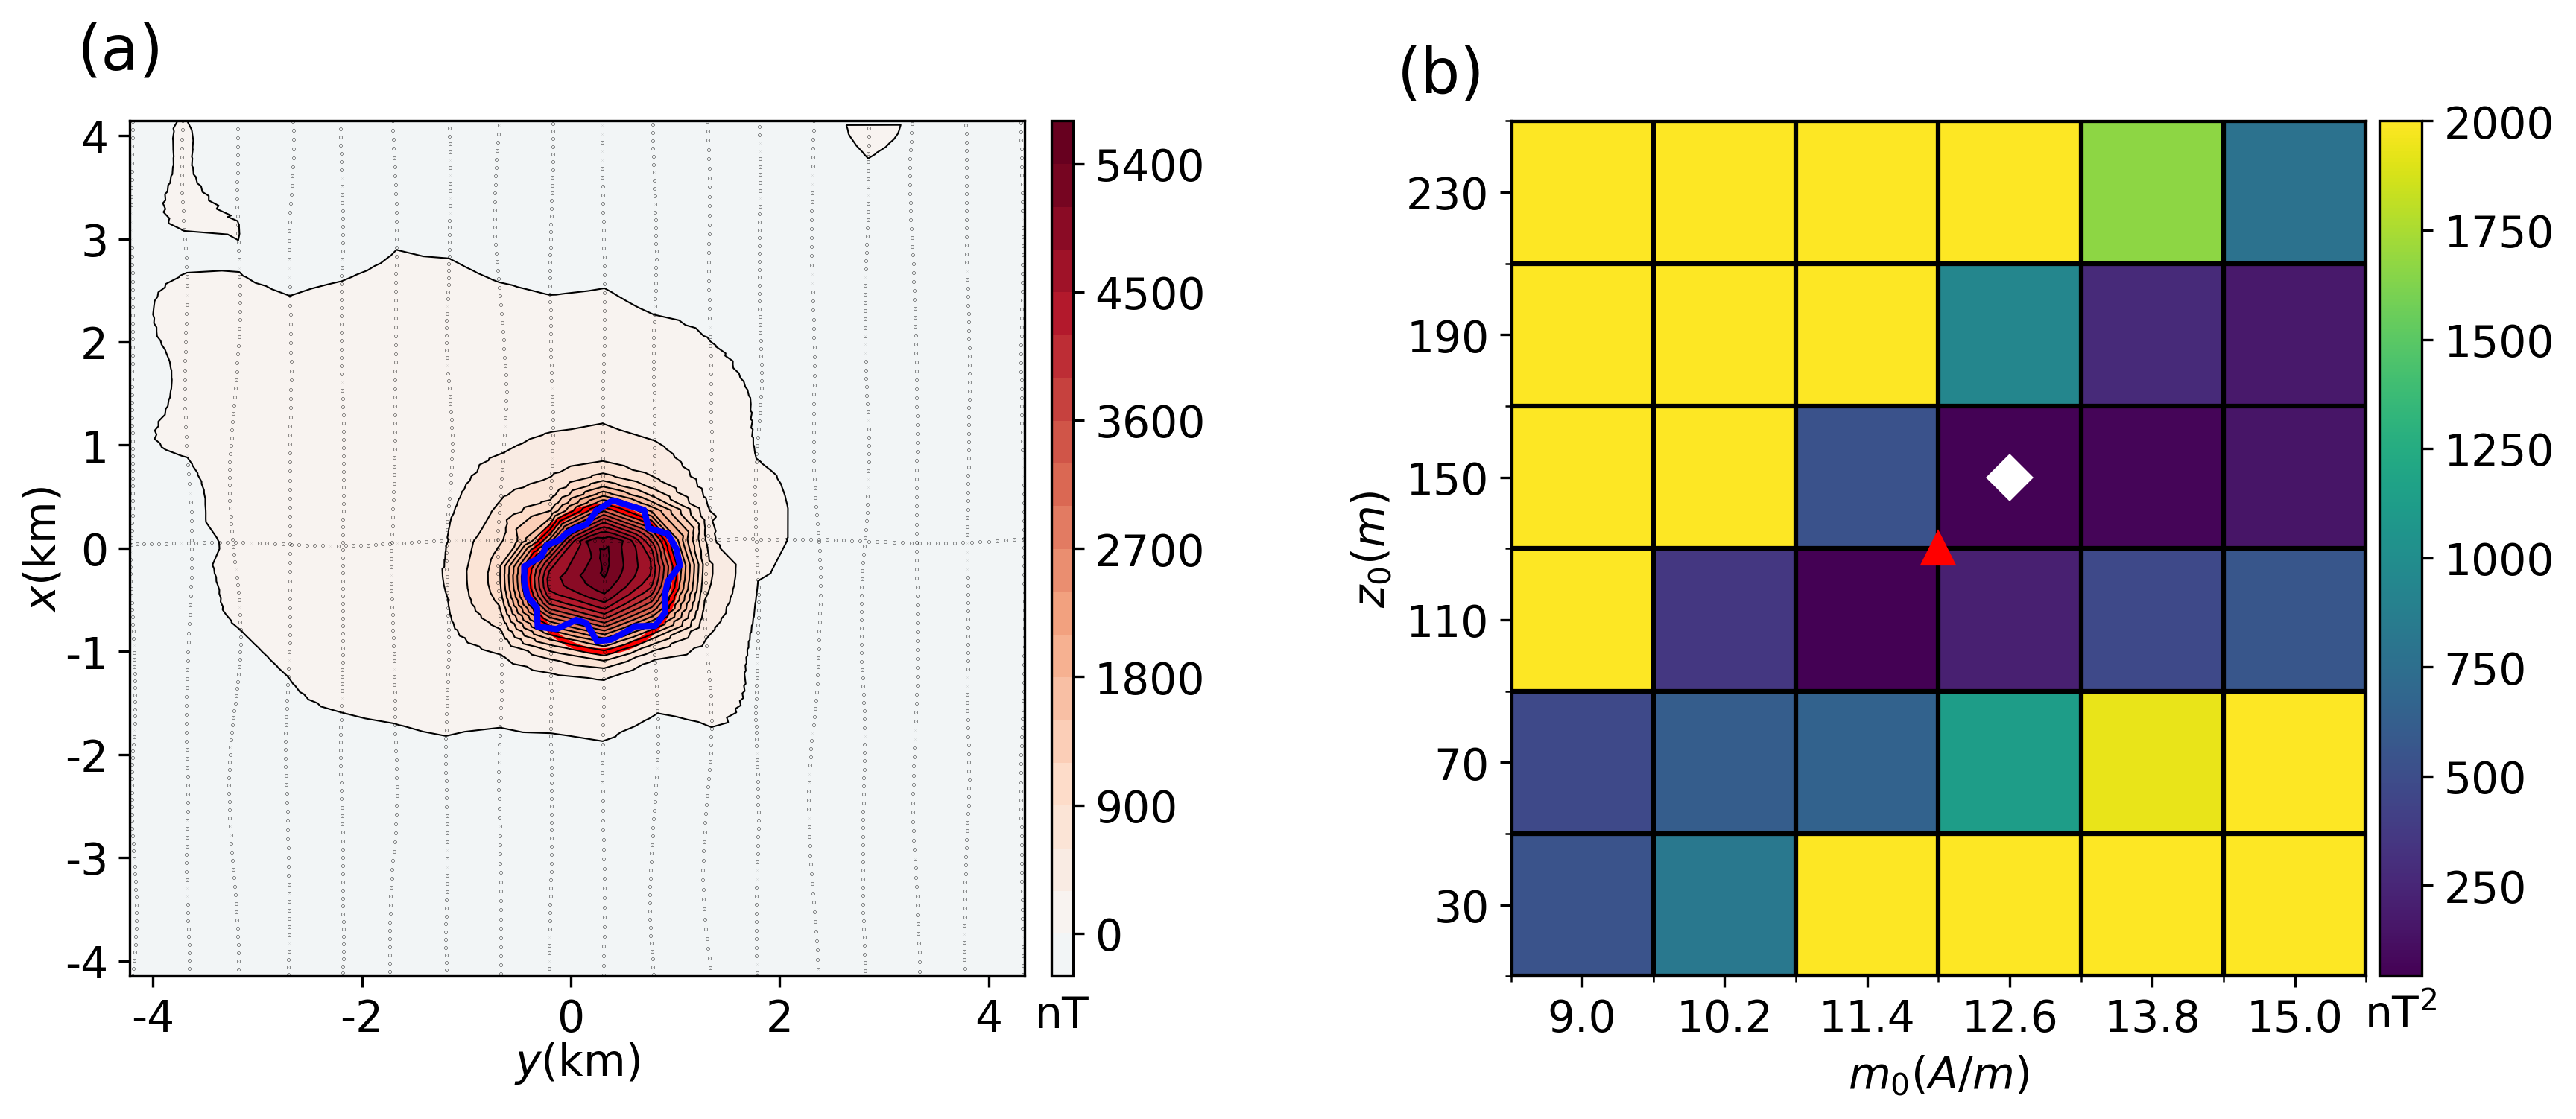
\includegraphics[width=\linewidth]{figures/complex_rtp.png}
    \caption{Complex model simulation. (a) RTP anomaly of the total-field anomaly
    shown in Fig. \ref{fig:complex_model}(a). 
	The red circle and the blue polygon represent the horizontal projections of the
	initial approximation $\hat{\mathbf{p}}_{(0)}$ and  the simulated dipping source,
	respectively.
	(b) Discrete map of the goal function $\Gamma(\mathbf{p}, m_0, z_0)$ (Eq.
	\ref{eq:gamma}) produced by the estimates $\hat{\mathbf{p}}_{(f)}$ obtained with
	a $6 \times 6$ grid of tentative values for depth to the top $z_0$ and
	total-magnetization intensity $m_0$.
	The red triangle and white diamond pinpoint, respectively, the true and
	retrieved values of $m_0$ and $z_0$.     
}
    \label{fig:complex_rtp}
\end{figure}

\begin{figure}
    \centering
    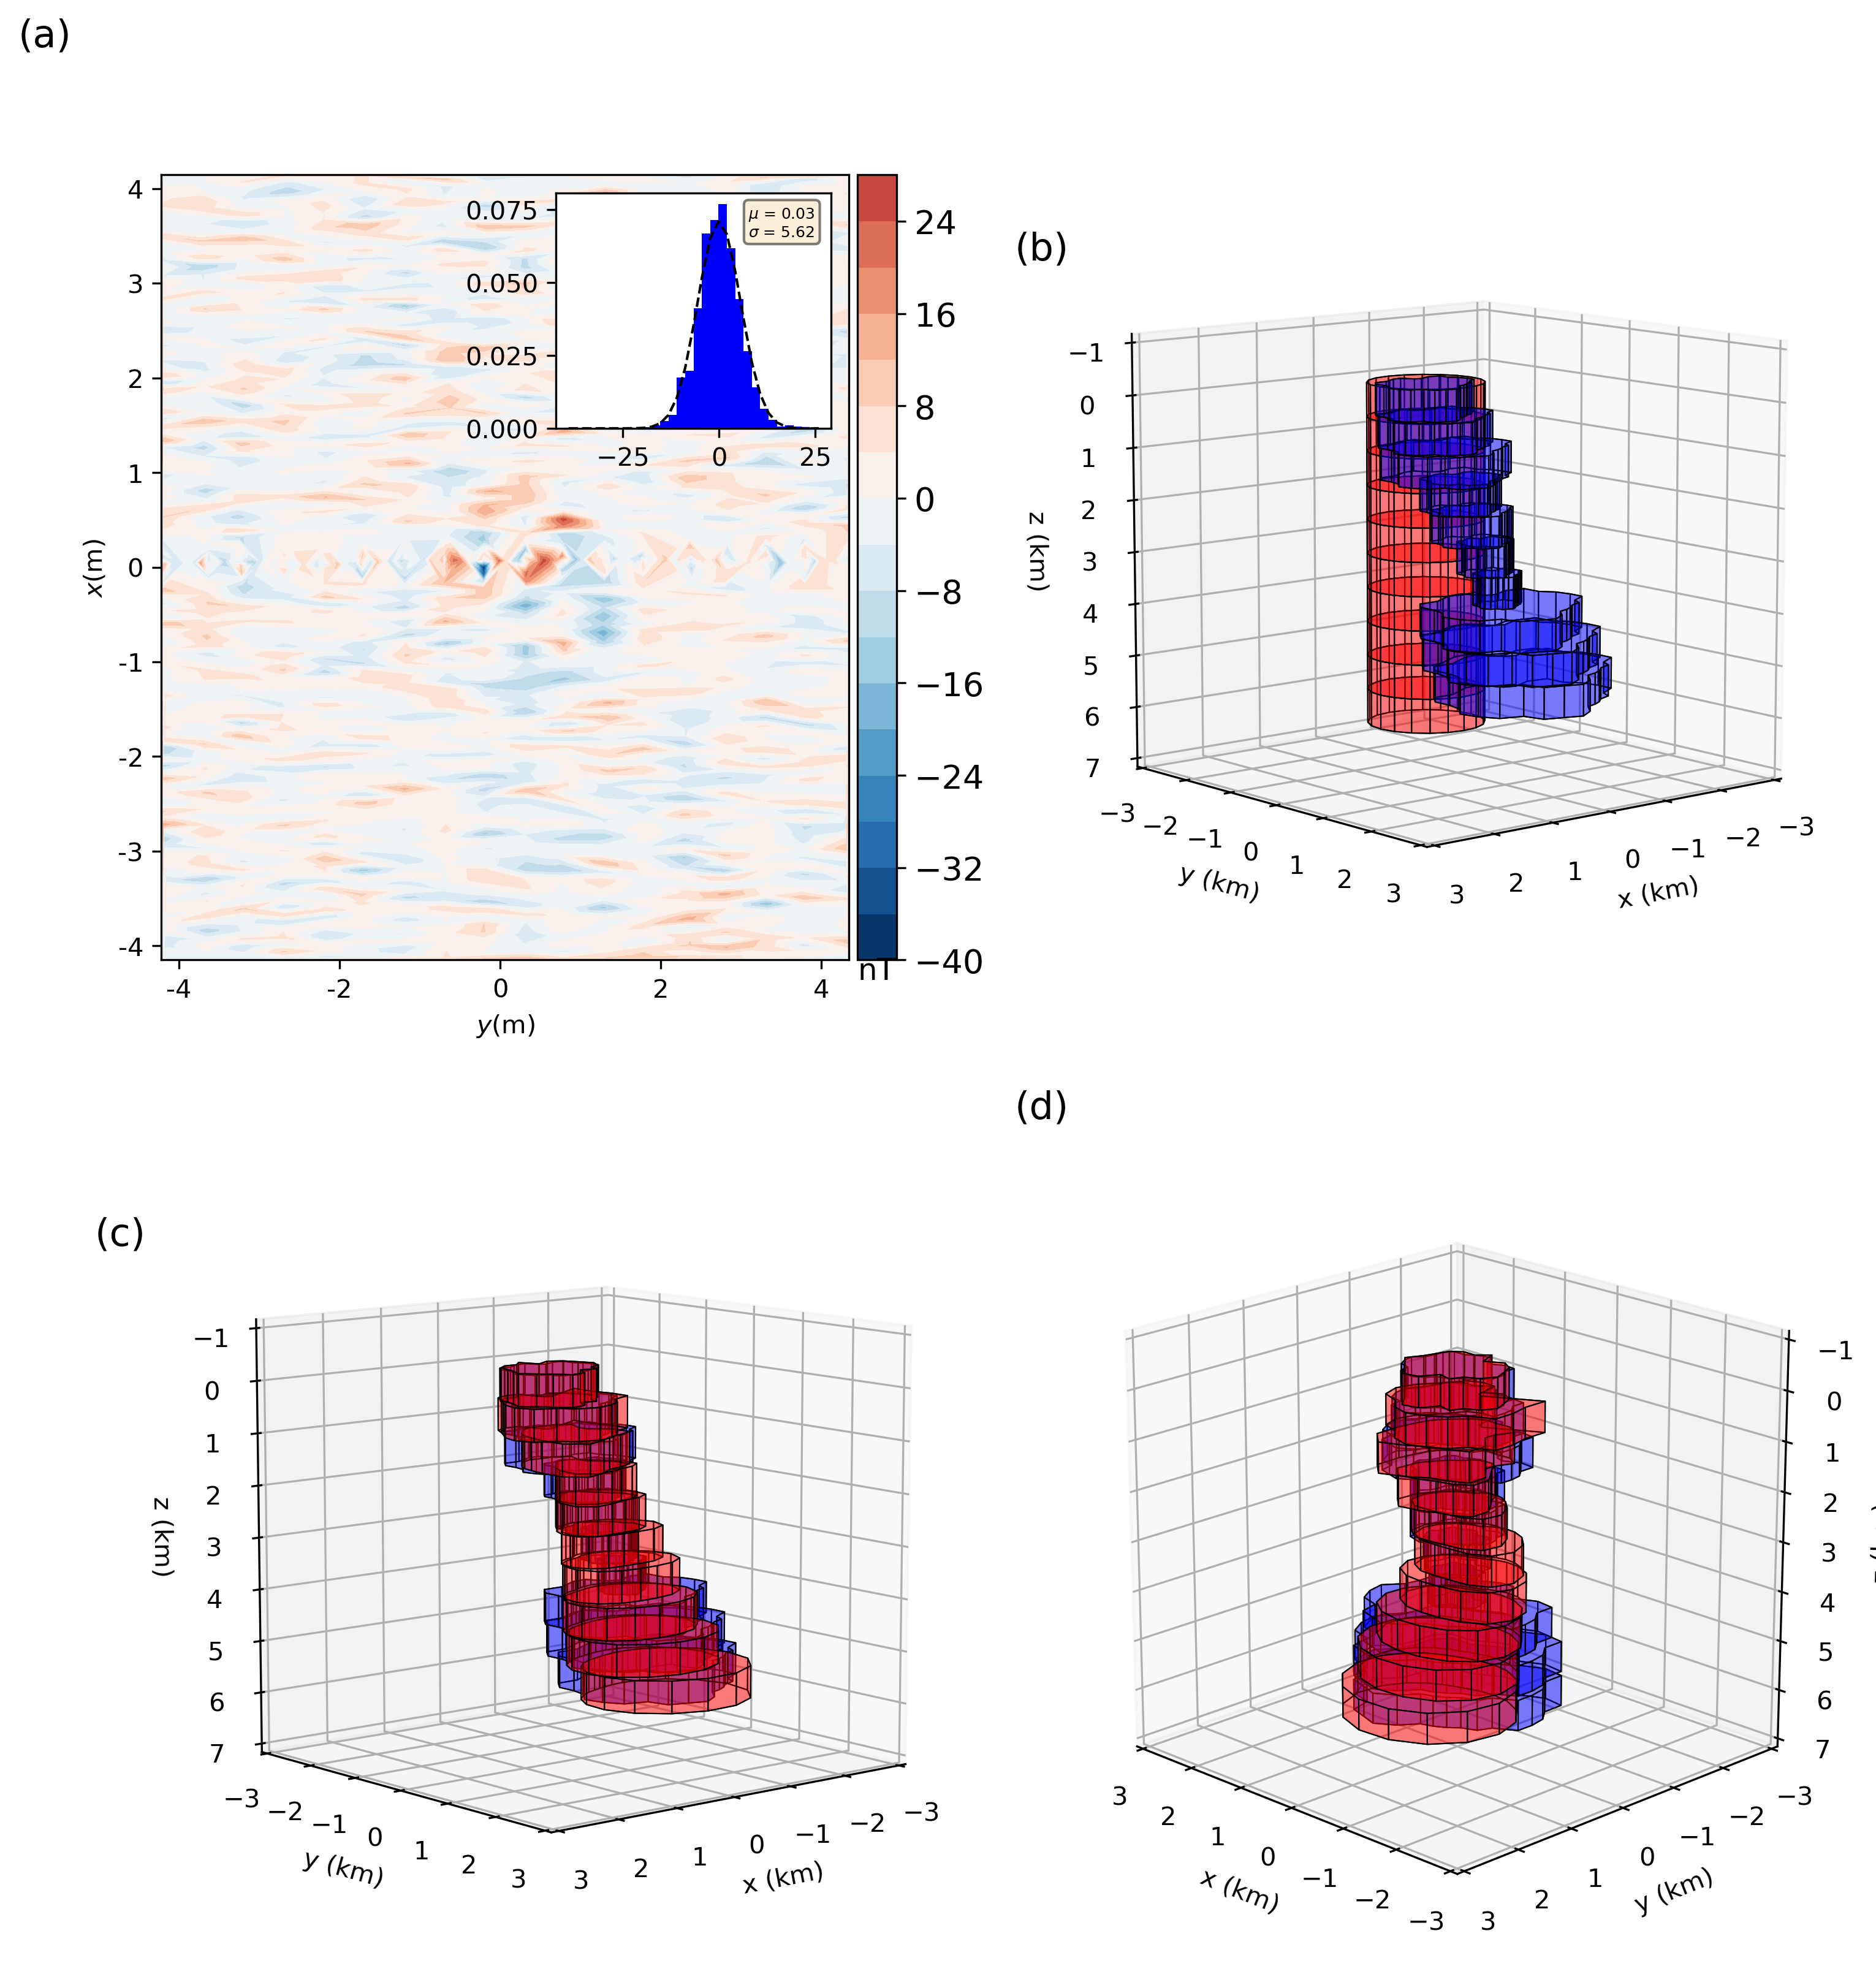
\includegraphics[width=\linewidth]{figures/complex_results.png}
    \caption{Complex model simulation. (a) Residuals between the noise-corrupted data (Fig. \ref{fig:complex_model}a) and the predicted data (not shown) produced by the estimated model (red prisms panels (c) and (d)) using $m_0$  and $z_0$ pinpointed by the white diamond in Fig. \ref{fig:complex_rtp}b.
    The inset shows the histogram of the residuals and the Gaussian curve (dashed line) has mean and standard deviation equal to $\mu = 0.01$ nT and $\sigma=6.6$ nT, respectively.  (b) Perspective view of the initial approximation (red prisms) and the true model (blue prisms). (c) and (d) Comparison between the estimated source (red prisms) and the true model (blue prisms) in perspective views. 
}
    \label{fig:complex_result}
\end{figure}

% Application to field data

\begin{figure}
    \centering
    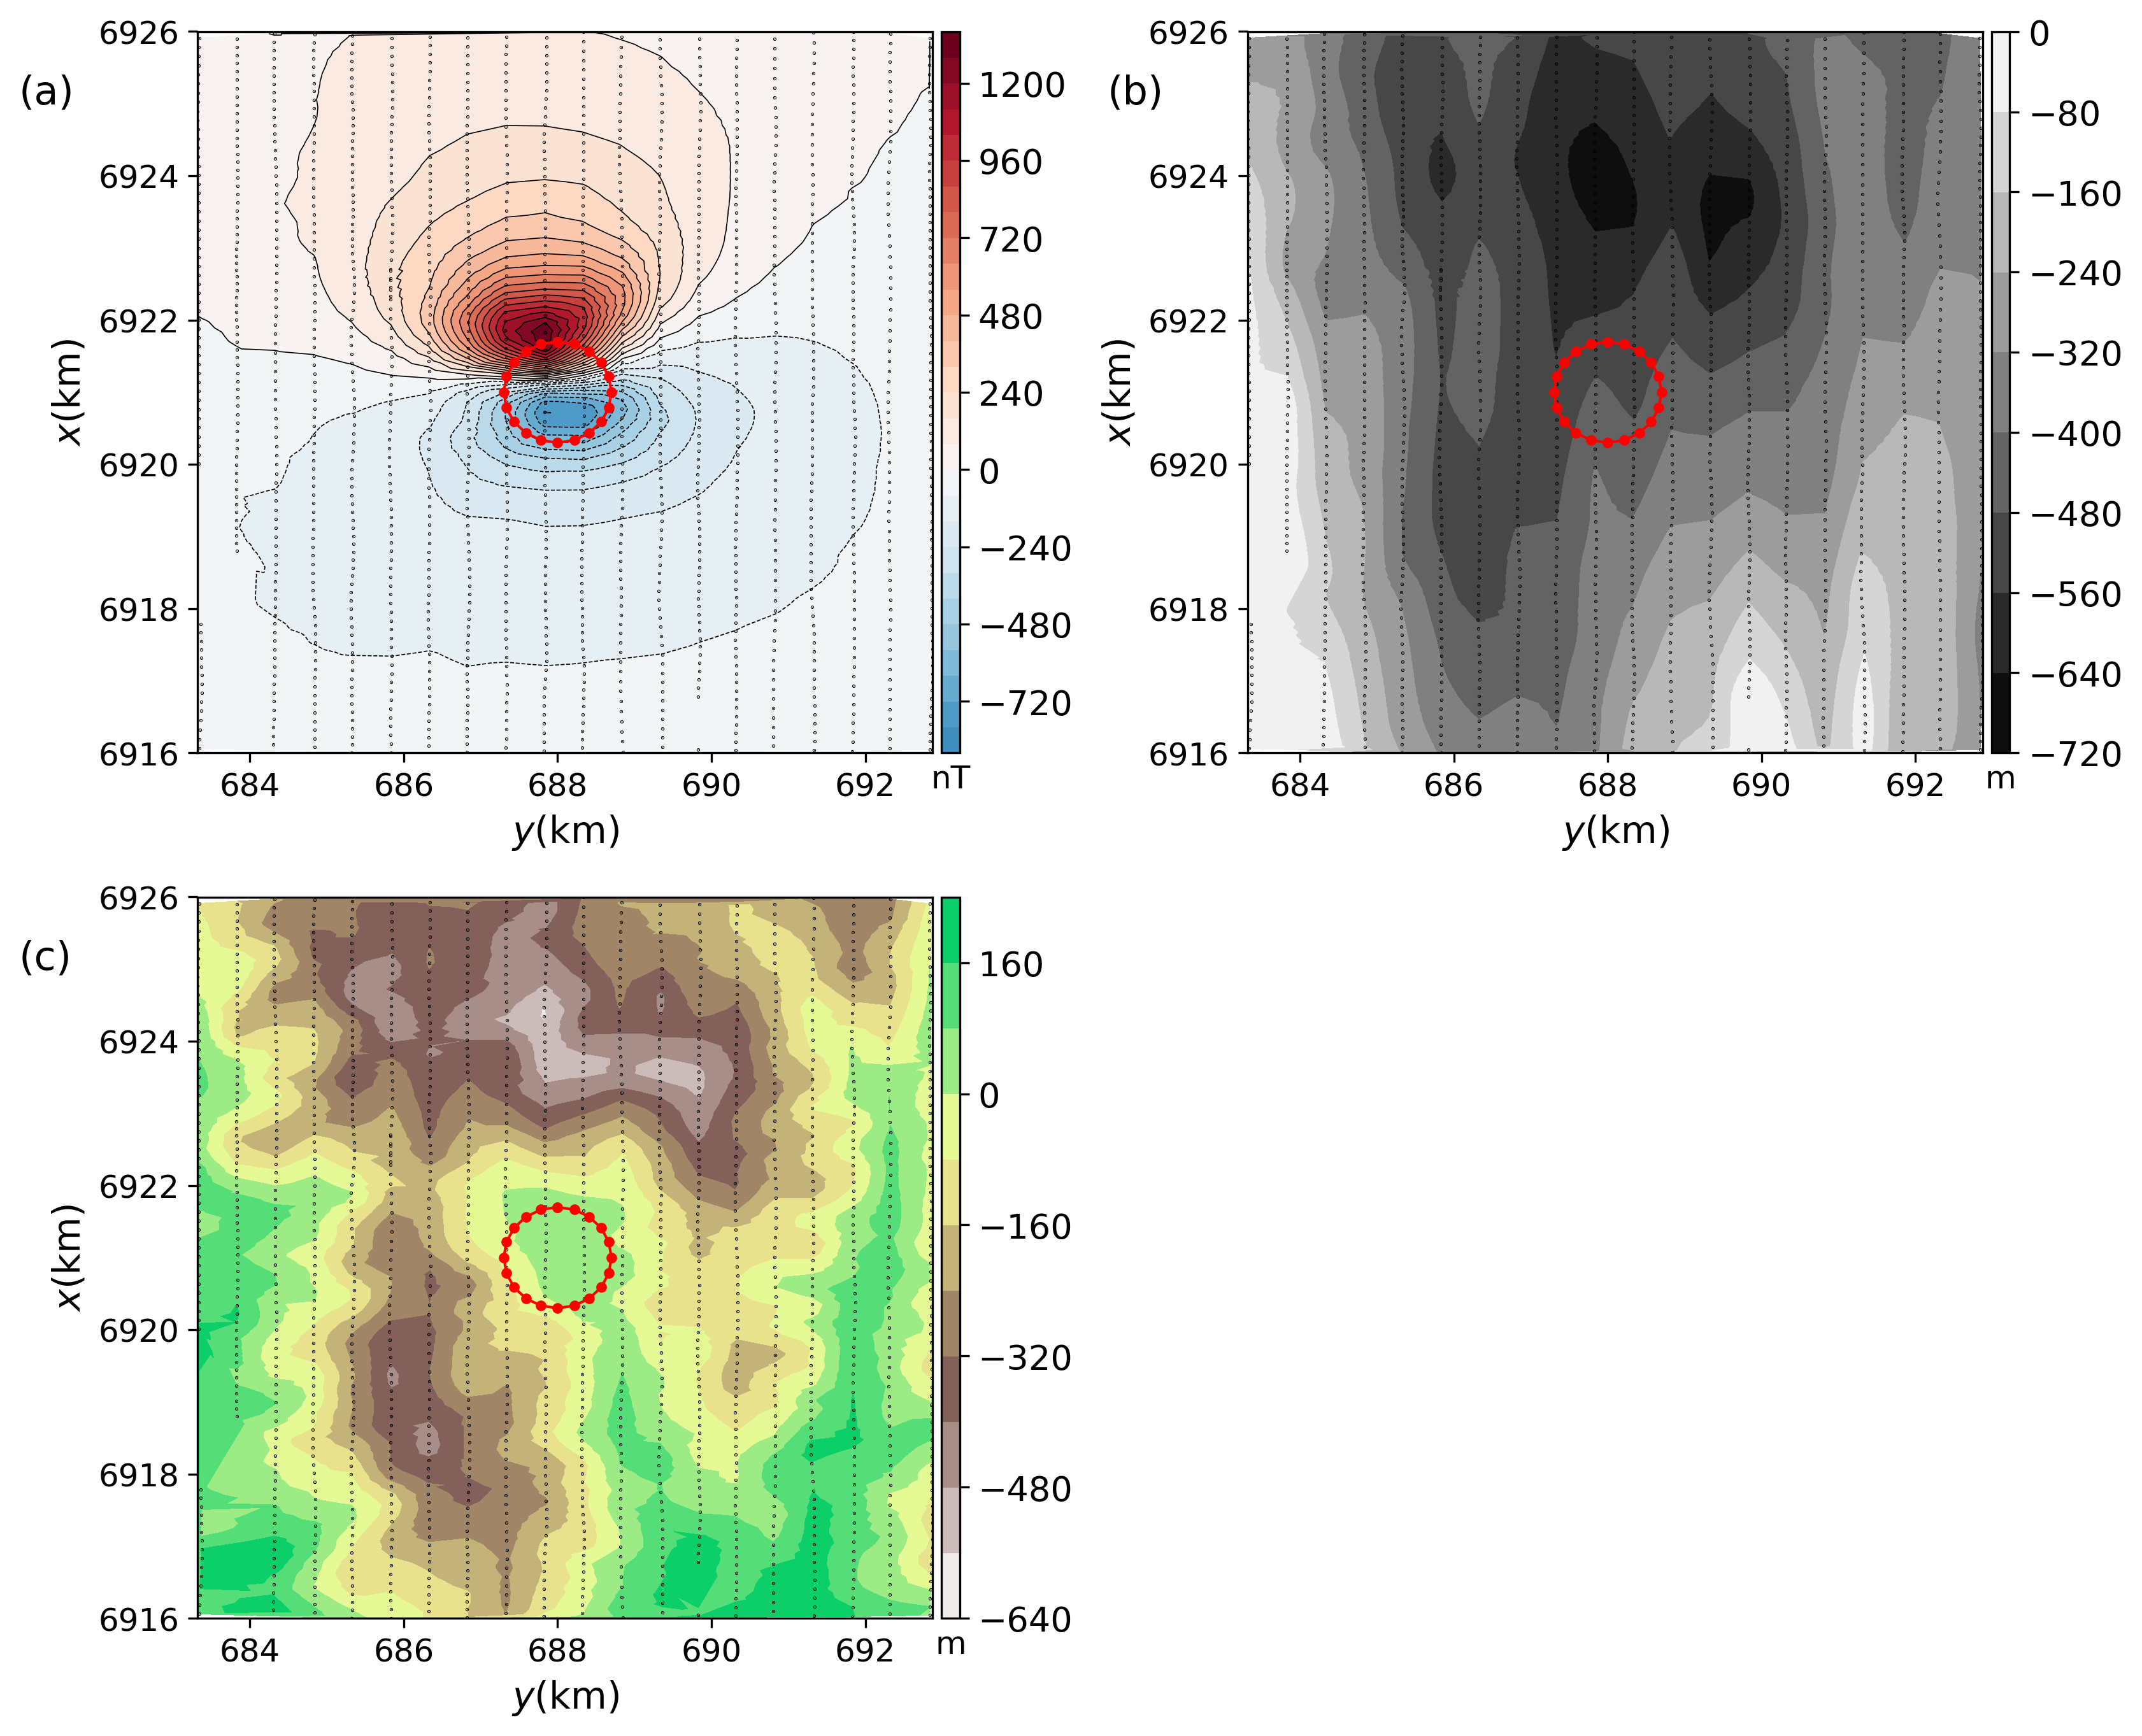
\includegraphics[width=\linewidth]{figures/field_data_alt_topo.png}
    \caption{Application to field data.  (a) Observed total-field anomaly over the  
    Anit{\'a}polis alkaline-carbonatitic complex in southern Brazil. The horizontal UTM 
    coordinates are referred to the central meridian $ 51^\circ $ W. 
    The black dots represent the observation points.
    (b) Regional field using least-squares first-order polynomial fitting. 
    (c) Geometric height of the observation points. (d) Topography of the study area.
    Both of these coordinates are referred to the WGS84 ellipsoid. We have subtracted 
    $ 800 $ m from their values. 
    The magenta rectangle delimits the data to be inverted.
    }
    \label{fig:real_data}
\end{figure}

\begin{figure}
    \centering
    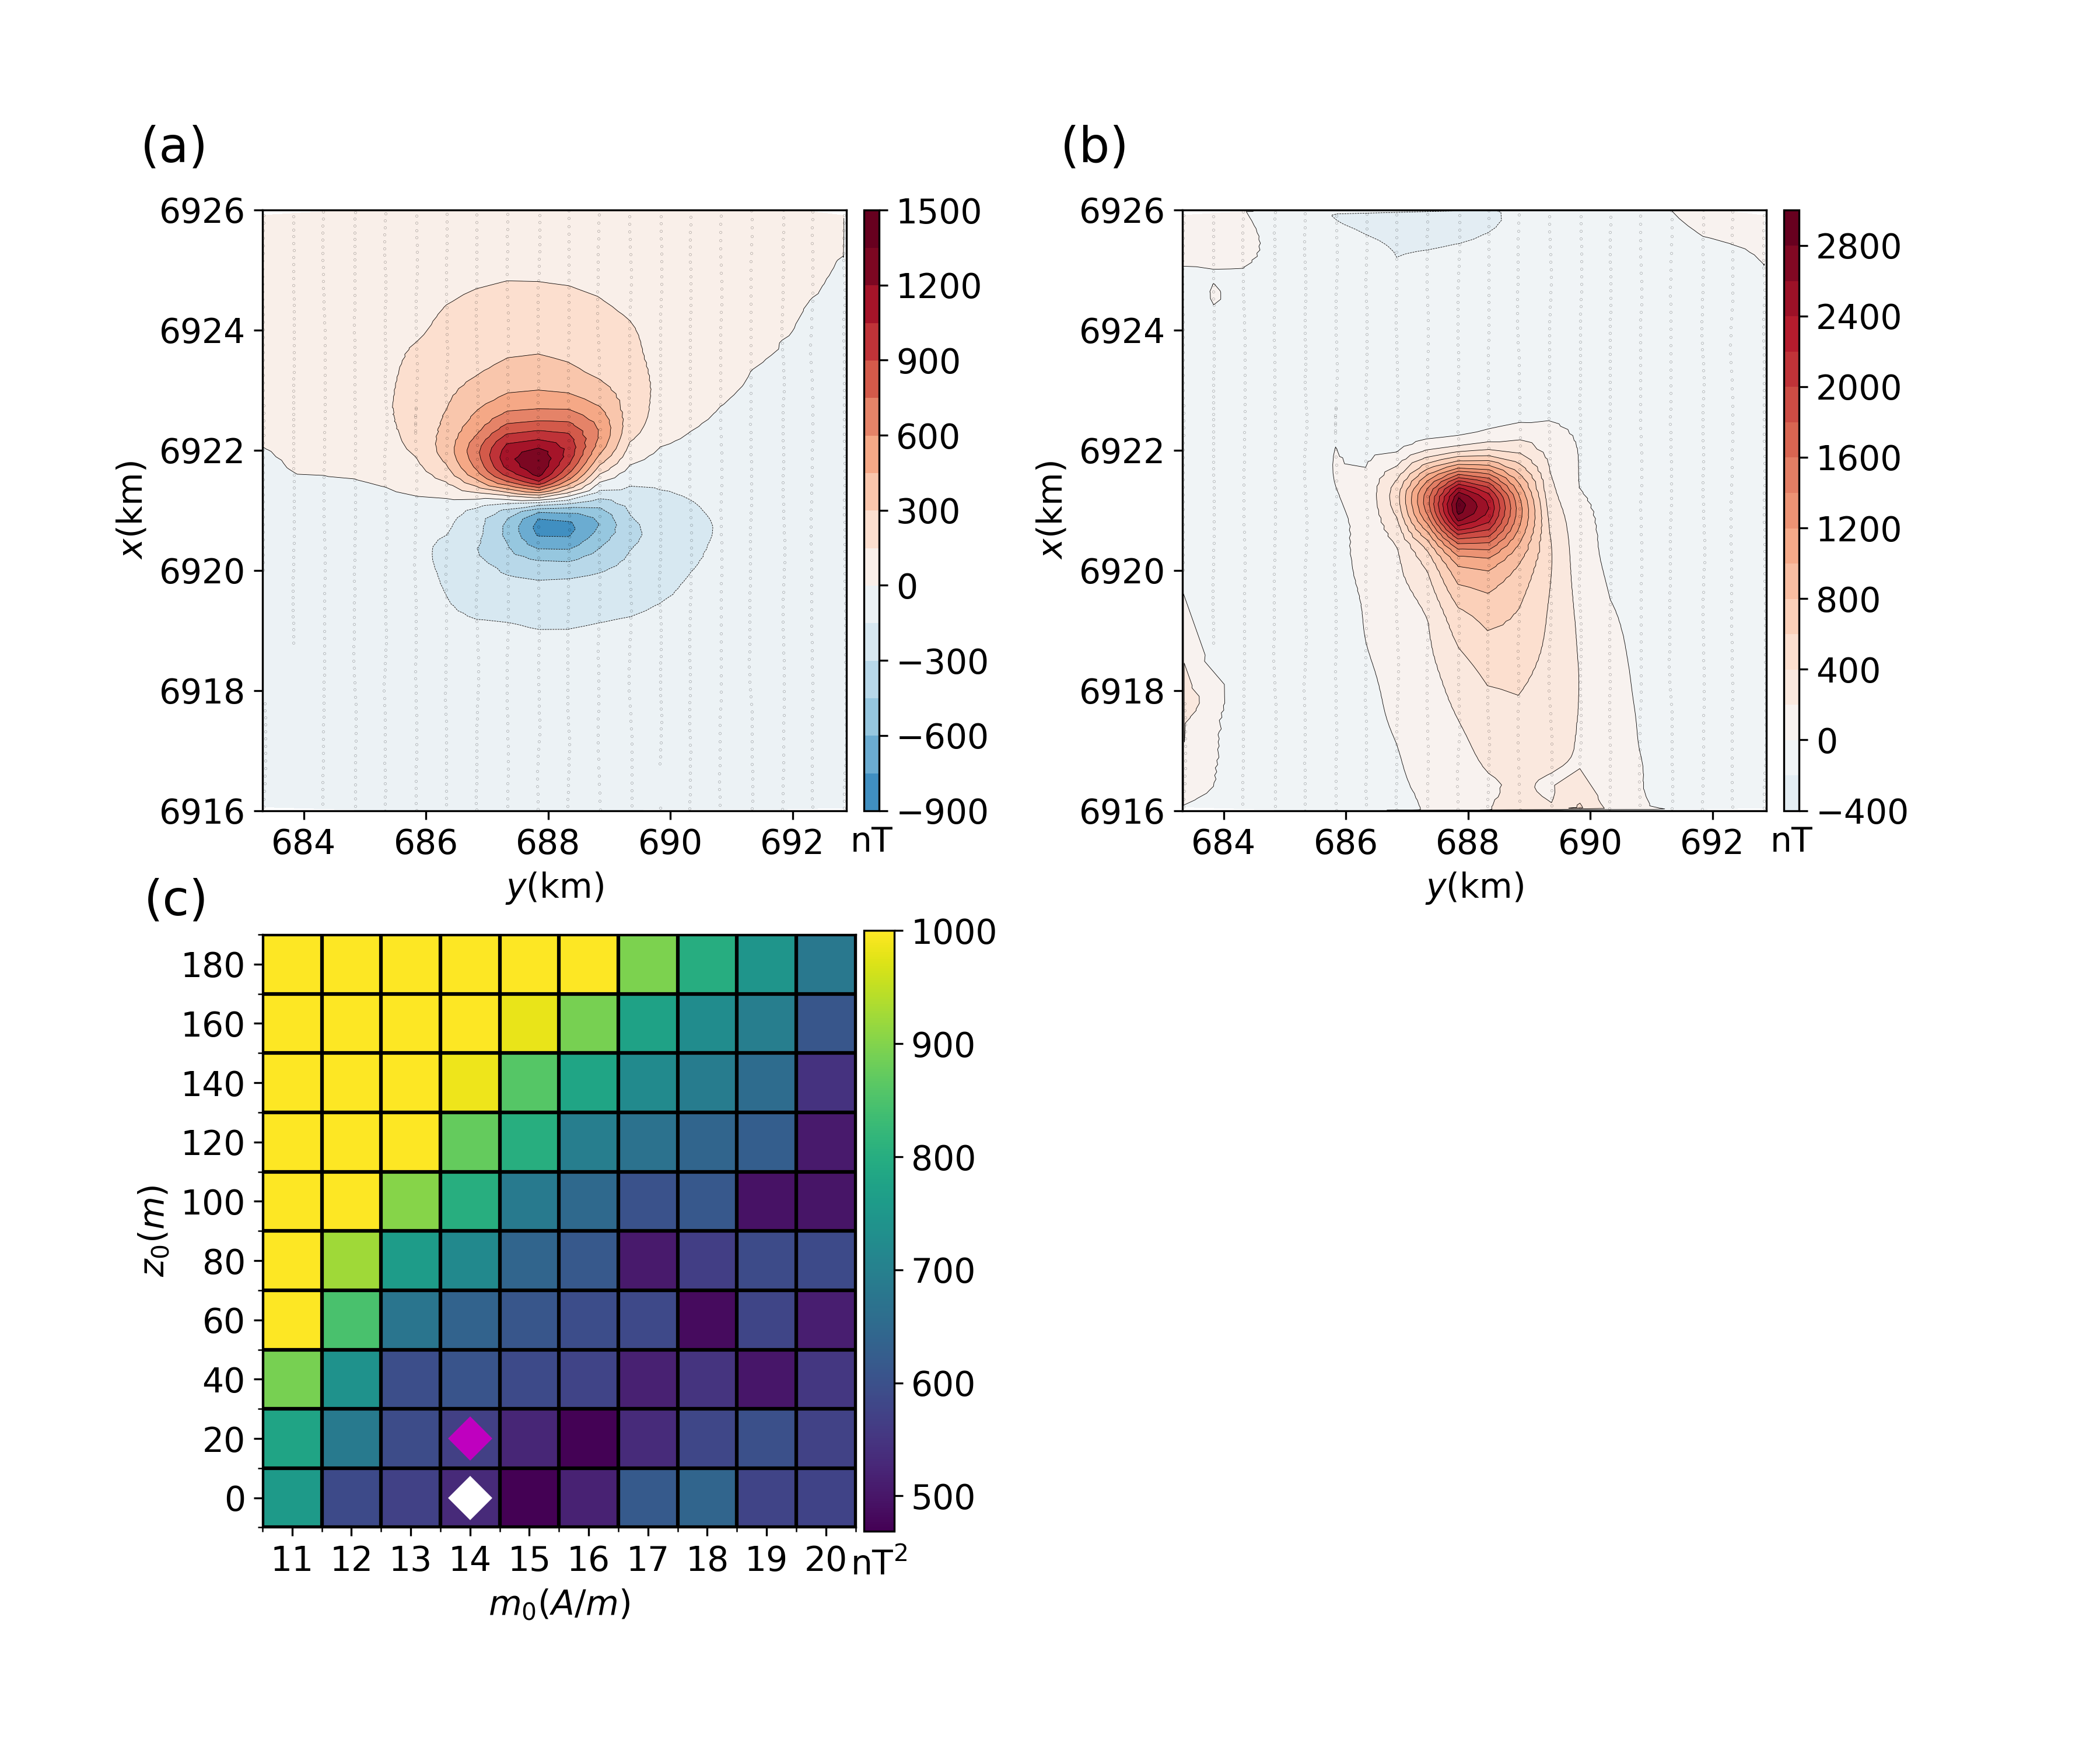
\includegraphics[width=\linewidth]{figures/anitapolis_rtp.png}
    \caption{Application to field data over the Anit{\'a}polis complex, Brazil. 
    (a) Residual total-field anomaly to be inverted over the area delimited by the 
    magenta rectangle in Fig. \ref{fig:real_data}. The red circle represents the
    horizontal projections of the initial approximation $\hat{\mathbf{p}}_{(0)}$.
    (b) RTP anomaly of the  residual total-field anomaly shown in panel (a).
    (c) Discrete map of the goal function $\Gamma(\mathbf{p}, m_0, z_0)$ (Eq.
    \ref{eq:gamma}) produced by the estimates $\hat{\mathbf{p}}_{(f)}$ obtained with
    a $6 \times 6$ grid of tentative values for depth to the top $z_0$ and
    total-magnetization intensity $m_0$.
    The white and magenta diamonds pinpoint, respectively, two pairs of $m_0$ and
    $z_0$ whose goal functions are close to each other. The magenta diamond pinpoints the estimated model that produces the smallest value of 
    $\Gamma(\hat{\mathbf{p}}_{(f)}, m_0, z_0)$.
    The white diamond pinpoints an alternative model whose depth to the top is $z_0=0$ indicating a possible outcropping not corroborated by the literature.	 
}
    \label{fig:anitapolis_rtp}
\end{figure}



\begin{figure}
	\centering
	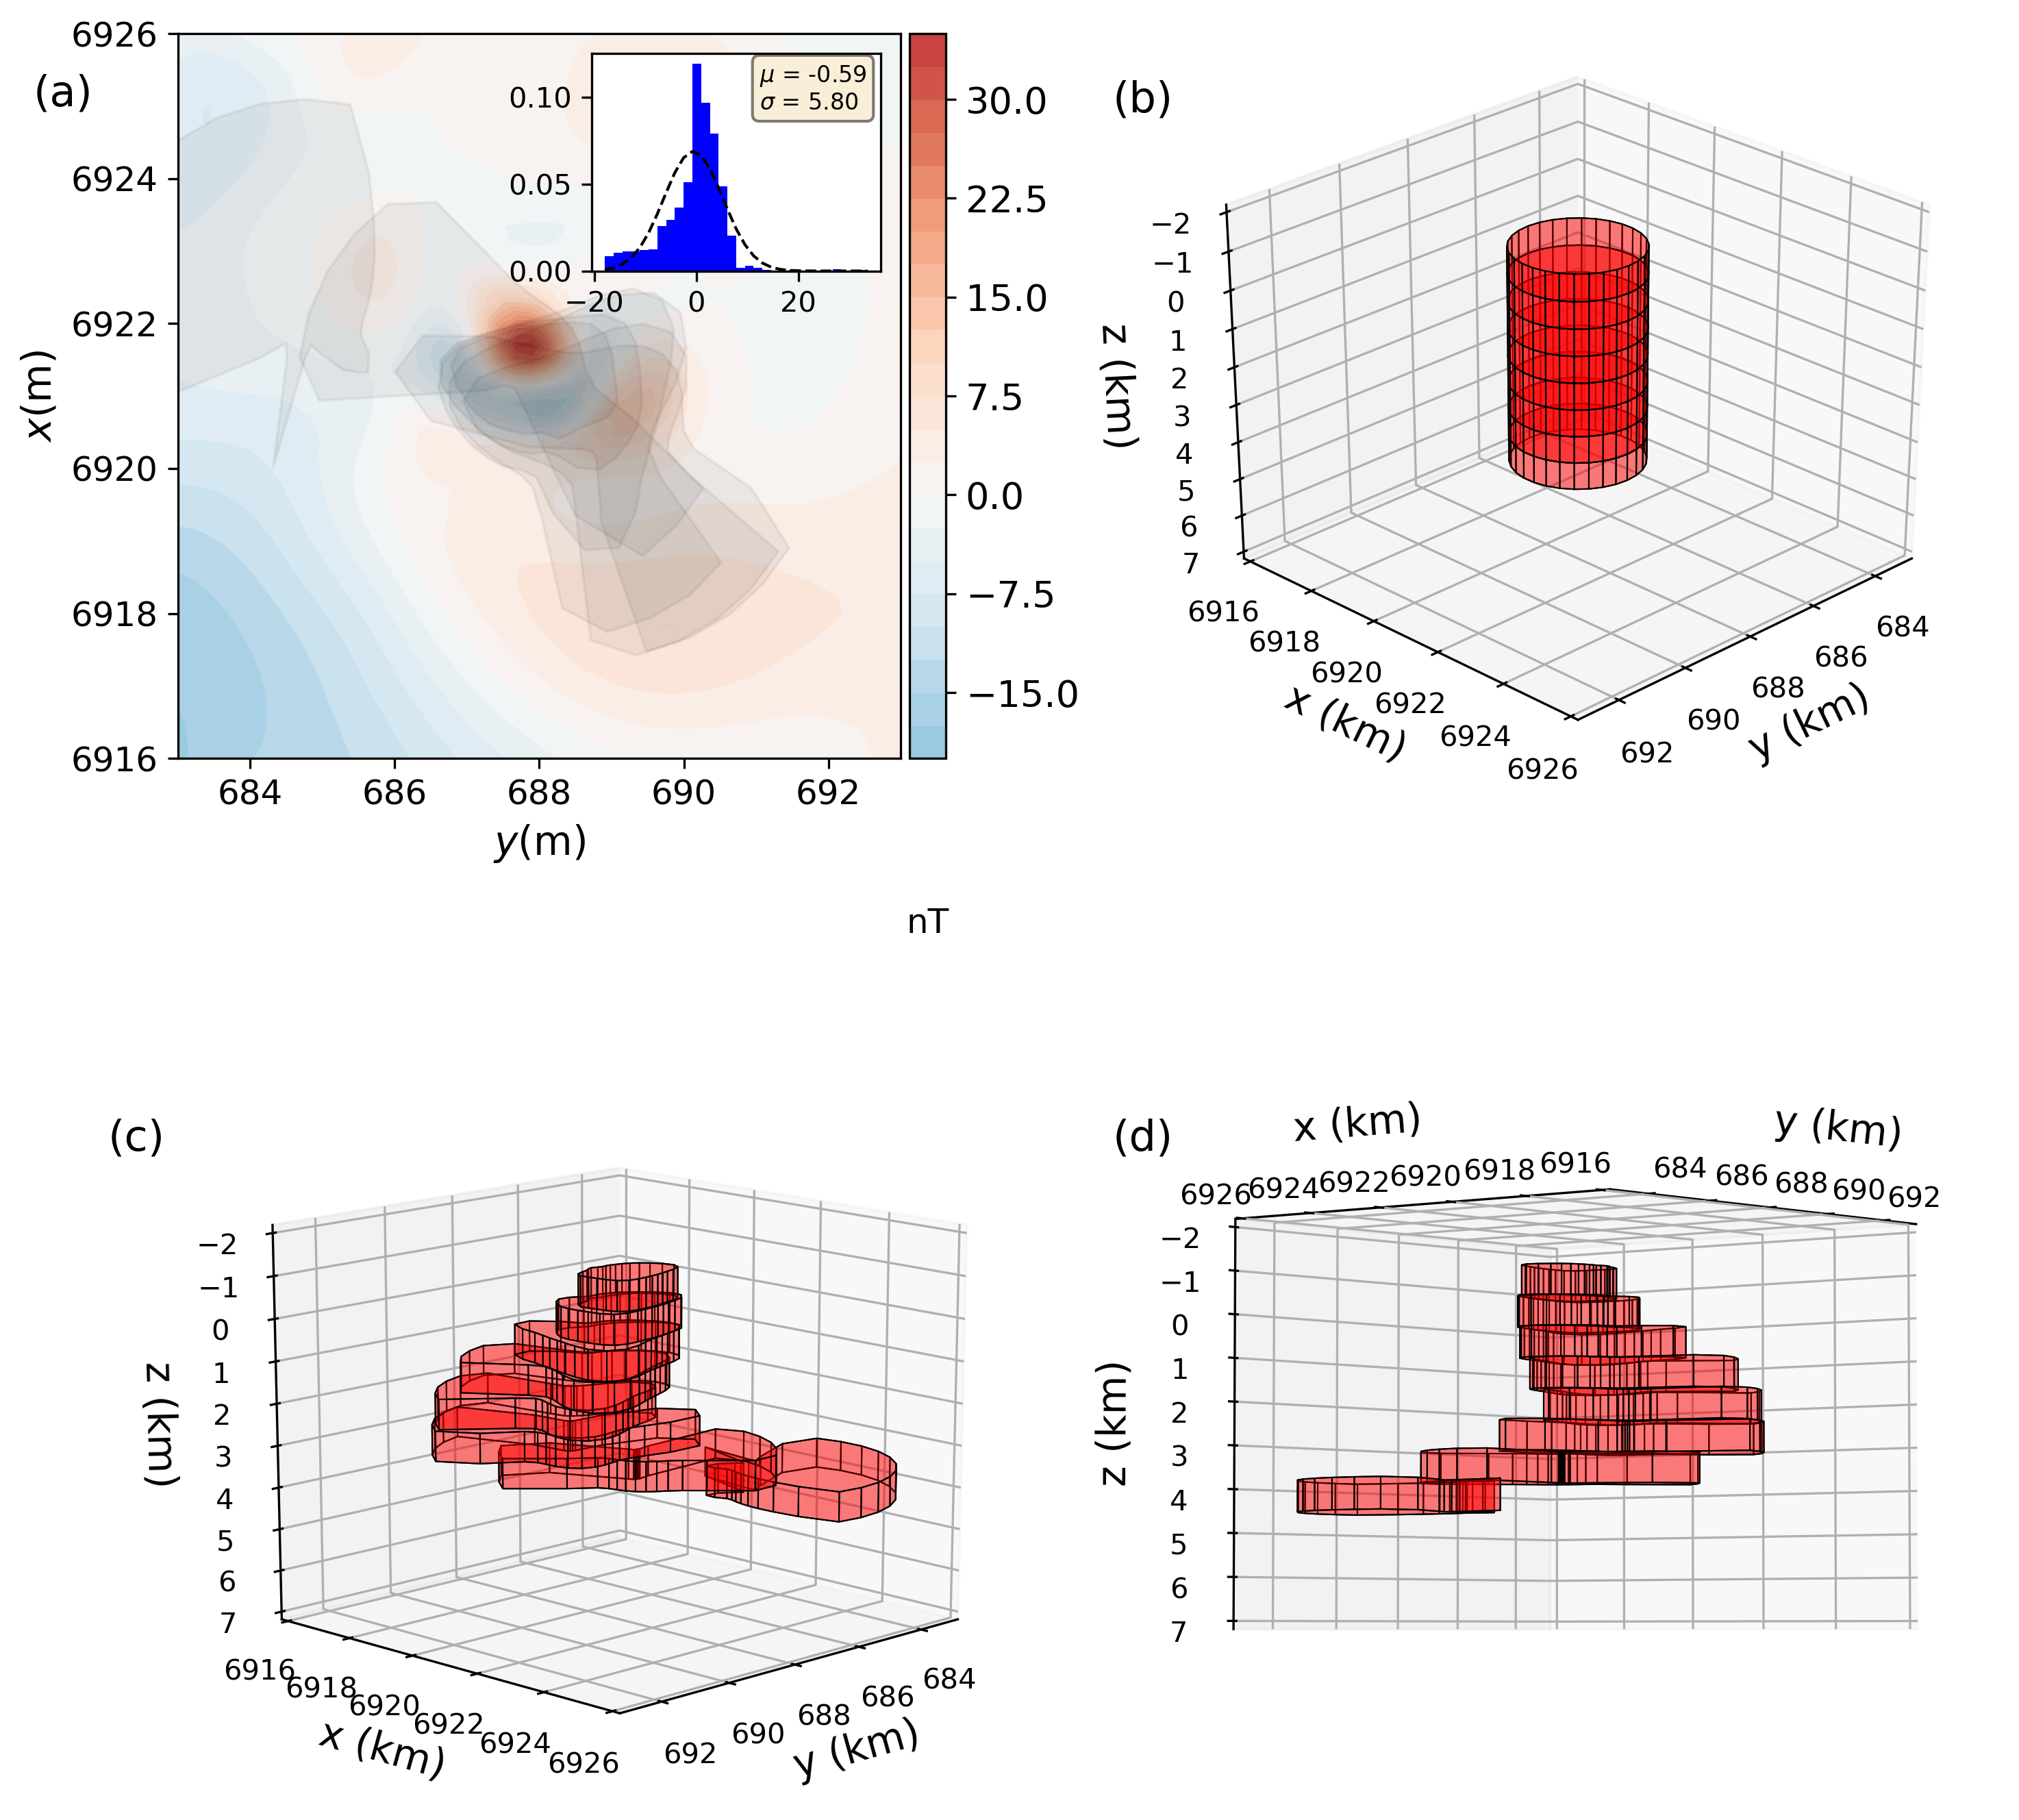
\includegraphics[width=\linewidth]{figures/real_results_magenta_diamond.png}
	\caption{Application to the field data over the Anit{\'a}polis complex, Brazil.
	The non-outcropping estimated model producing the smallest goal function 
	($ \Gamma(\hat{\mathbf{p}}_{(f)}, m_0, z_0)$, Eq. \ref{eq:gamma})	represented by the magenta diamond 
	in Fig. \ref{fig:anitapolis_rtp}c.
	(a) Residuals between the observed data (Fig. \ref{fig:anitapolis_rtp}a) and the 
	predicted data (not shown) produced by the estimated model. 
	The inset shows the histogram of the residuals and the fitted normal 
	Gaussian curve (dashed line) with mean $\mu = -1.2$ nT and 
	standard deviation $\sigma = 20.70$ nT.
	The light-gray polygons represent the horizontal projection of the estimated 
	model onto the residual map. 
	(b) Perspective view of the initial approximation (red prisms). 
	(c) and (d) Perspective views of the estimated model (red prisms).}
	\label{fig:real_result2}
\end{figure}

\begin{figure}
    \centering
    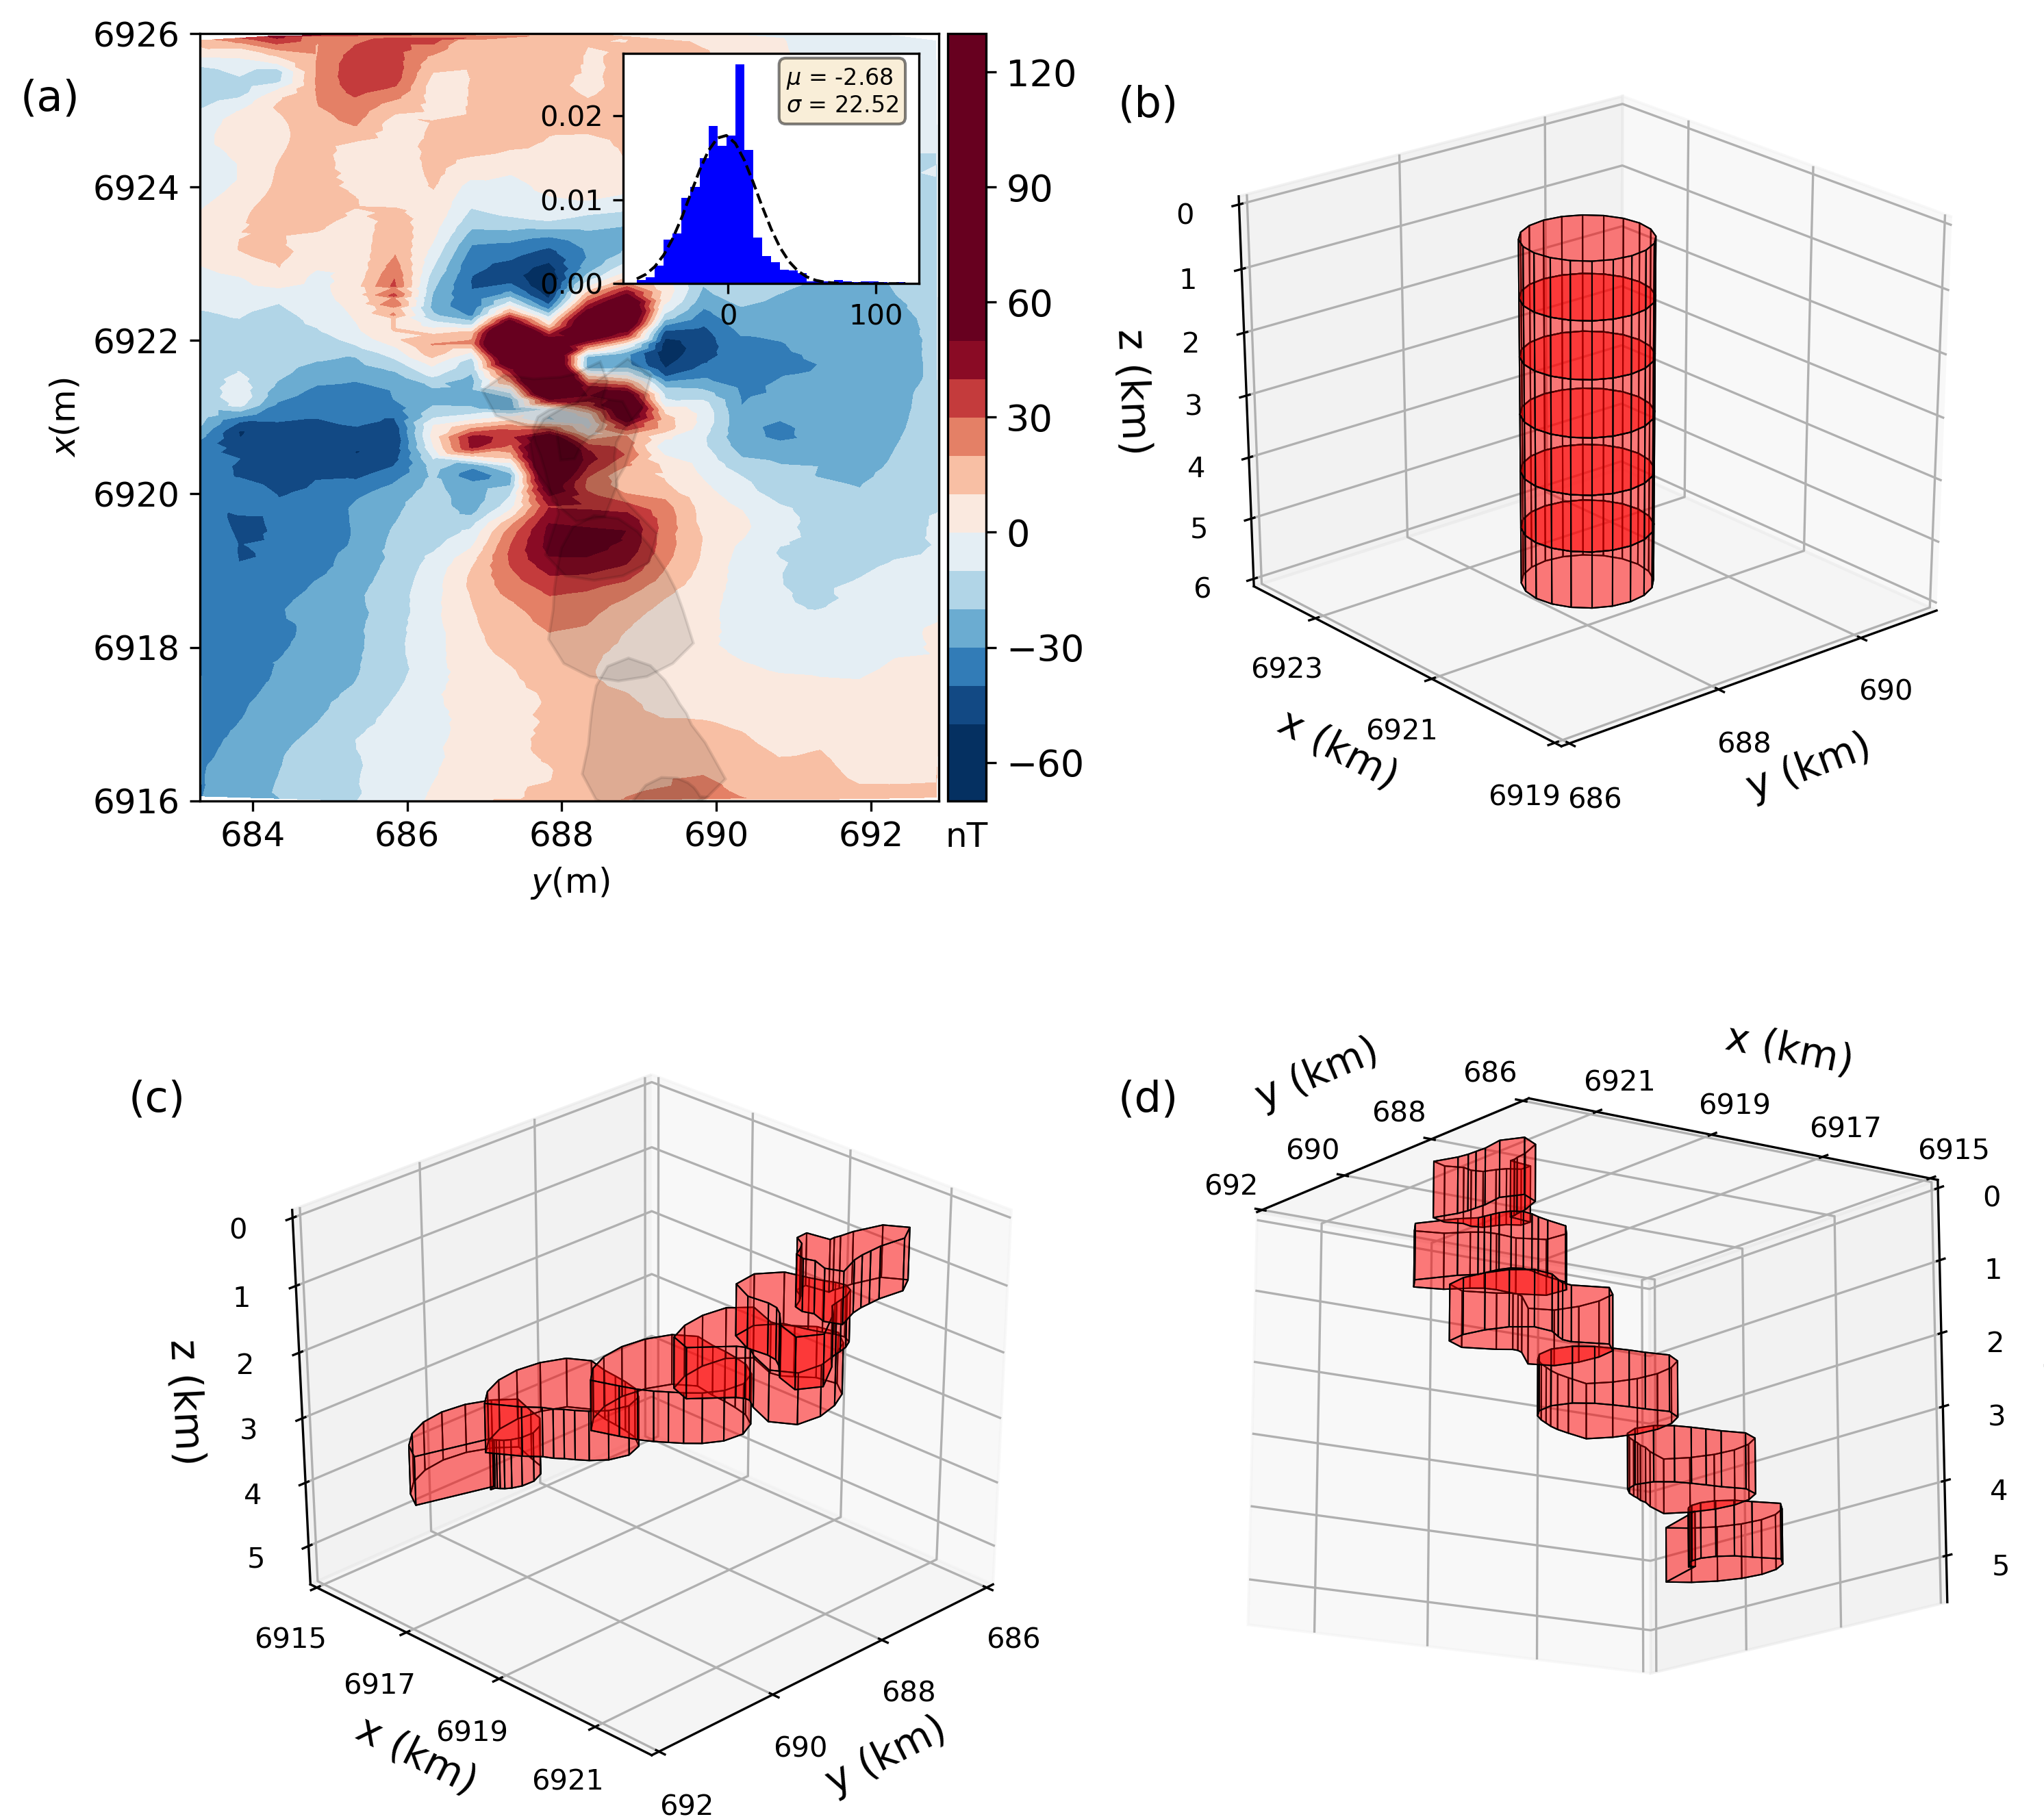
\includegraphics[width=\linewidth]{figures/real_results_white_diamond.png}
    \caption{Application to the field data over the Anit{\'a}polis complex, Brazil.
    Outcropping estimated model  represented by the white diamond in in Fig.    		   \ref{fig:anitapolis_rtp}c. 
    (a) Residuals between the observed data (Fig. \ref{fig:anitapolis_rtp}a and the 
    predicted data (not shown) produced by the estimated model. 
    The inset shows the histogram of the residuals and the fitted normal 
    Gaussian curve (dashed line) with mean $\mu = 1.0$ and standard deviation  
    $\sigma = 20.6$.
    The light-gray polygons represent the horizontal projection of the estimated 
    model onto the residual map. 
    (b) Perspective view of the initial approximation (red prisms). 
    (c) and (d) Perspective views of the estimated model (red prisms).}
    \label{fig:real_result}
\end{figure}